%%%%%%%%%%%%%%%%%%%%%%%%%%%%%%%%%%%%%%%%%
% Simple Sectioned Essay Template
% LaTeX Template
%
% This template has been downloaded from:
% http://www.latextemplates.com
%
% Note:
% The \lipsum[#] commands throughout this template generate dummy text
% to fill the template out. These commands should all be removed when 
% writing essay content.
%
%%%%%%%%%%%%%%%%%%%%%%%%%%%%%%%%%%%%%%%%%

%----------------------------------------------------------------------------------------
%	PACKAGES AND OTHER DOCUMENT CONFIGURATIONS
%----------------------------------------------------------------------------------------

\documentclass[10pt]{book} % Default font size is 12pt, it can be changed here

\usepackage{geometry} % Required to change the page size to A4
\geometry{a4paper} % Set the page size to be A4 as opposed to the default US Letter

\usepackage{graphicx} % Required for including pictures

\usepackage{float} % Allows putting an [H] in \begin{figure} to specify the exact location of the figure
\usepackage{wrapfig} % Allows in-line images such as the example fish picture

\usepackage{multibbl}
\usepackage{hyperref}
\usepackage{amsmath,gensymb}

\usepackage{pdfpages}

\linespread{1.5} % Line spacing

%\setlength\parindent{0pt} % Uncomment to remove all indentation from paragraphs

\graphicspath{{Pictures/}} % Specifies the directory where pictures are stored

\begin{document}

%----------------------------------------------------------------------------------------
%	TITLE PAGE
%----------------------------------------------------------------------------------------

\begin{titlepage}

\newcommand{\HRule}{\rule{\linewidth}{0.5mm}} % Defines a new command for the horizontal lines, change thickness here

\center % Center everything on the page

\textsc{\LARGE University of Tennessee, Knoxville}\\[1.5cm] % Name of your university/college
\textsc{\Large ESE 512: Pricing and Policy}\\[0.5cm] % Major heading such as course name

\HRule \\[0.4cm]
{ \huge \bfseries Creating a Solar Market}\\[0.4cm] % Title of your document
\HRule \\[1.5cm]

\textsc{\large Jay Jay Billings, Julie Cease, Roisin Langan, Eric Muckley,
Patrick Shower and Deborah Weighill}\\[0.5cm] % Minor heading such as course title





{\large \today}\\[3cm] % Date, change the \today to a set date if you want to be precise

%\includegraphics{Logo}\\[1cm] % Include a department/university logo - this will require the graphicx package



\end{titlepage}

%----------------------------------------------------------------------------------------
%	TABLE OF CONTENTS
%----------------------------------------------------------------------------------------

%\tableofcontents % Include a table of contents


%----------------------------------------------------------------------------------------
%	INTRODUCTION
%----------------------------------------------------------------------------------------

\chapter{The Policy}

It is the recommendation of this project that the U.S. federal government 
create a strong solar energy market by outfitting and refitting federal
buildings with photovoltaics. Such a policy will ultimately save the government
directly in electricity costs and its carbon footprint, in spite of the the
significant technological challenges surrounding photovoltaics, especially
those related to intermittancy. In addition to the long-term savings to the
government, such a large scale roll out of photovoltaics would drive the price
of the technology lower without subsidies, thereby making solar energy
affordable for small businesses and families and further decreasing the
national carbon footprint.

We recommend, specifically, a two-fold policy applied to all states except
Alaska that
\begin{enumerate}
  \item all new government buildings entering the planning phase in
fiscal year 2017 be constructed with enough photovoltaics installed on their
roofs or on an equivalent square footage of adjacent land to off-set 30\% of
their electricity consumption from the power grid on a sunny day during peak
hours.
  \item all existing federal buildings undergo a refit by 2020 to install
photovoltaics on their existing roofs or on an equivalent square footage of
adjacent land to off-set 20\% of their electricity consumption from the
power grid on a sunny day during peak hours.
\end{enumerate}

We further recommend that the government pursue all types of photovoltaic
technology with the preference to type determined on what is best for the
facility in question and that the required efficiency of the chosen type be
determined through a certification program. The certification program would act
as a quality check to insure that all solar cells produced by the federal
government were within 10\% of the industry average efficiency for a given
type of photovoltaic, thus preventing the government from purchasing poor
equipment. After energy efficiency, the choice of photovoltaic cell must be
limited to those cells that are produced with a miminimal carbon intensity such
that the overall carbon footprint of the federal facility decreases.


\chapter{Justification}

% ----- Jay ----- %
\newbibliography{jay}
\section{Social Justice and Solar Energy: How Photovoltaics Can Help}
\textit{Jay Jay Billings}

The United States consumed 97.1 quadrillion BTUs of energy in 2013, nearly 
twenty percent of total global consumption \cite{jay}{eiaIntStats}. Likewise, the 
population of the United States is projected to hit nearly 417 million people 
by 2016 \cite{jay}{usCensus}. Rising energy costs over the next few decades will 
primarily affect the poor and the middle class since even large increases in 
the price of energy are a small percentage of the wages of the wealthy and 
there are so many lower income people in the United States relative to the 
wealthy. Likewise, if we continue to generate our future energy through 
traditional means it will not only mean that we have increased the income gap, 
but also our carbon footprint significantly because it such growth would be 
driven primarily driven by coal and natural gas. Thus, we need an alternative 
form of energy that is readily available, cheap, and overall quite clean. This 
paper will discuss these issues from the perspective of liberal nationalism and 
describe how photovoltaics may be the answer to providing affordable energy to 
those who need it most in such a framework.

\subsection{An Overview of US Energy}

Energy in the United States is primarily generated by three sources: fossil 
fuels, nuclear reactors and renewable energy \cite{jay}{eiaAEO2015}. Fossil fuels 
accounted for 81\% of the energy generated in 2013 with 27\%, 18\% and 36\% for 
\% natural gas, coal and petroleum respectively \cite{jay}{eiaAEO2015}. Roughly 74\%
of this energy was was for use as electricity with coal holding a slight 
majority over the other sources in 2013. The total cost of energy is expected 
to increase at a rate of 2.4\% per year between the 2013 and 2040 fiscal years 
while the total energy consumption will only grow at a rate of 0.9\% per year 
over the same period.

Natural gas is produced from either from its own wells or as a by-product from 
oil wells. Texas, Pennsylvania and Louisiana were the top three natural gas 
producing states in 2013, \cite{jay}{eiaAEO2015}. Coal is mined, either in deep 
underground mines or through strip mining and Wyoming, West Virginia and Kentucky 
were the top three coal producing states in 2013. Texas also consumed the most 
electricity in 2013, followed by California and Florida.

Renewable sources of energy accounted for 18\% of electricity generated in 2013 
and only 10\% of total energy generated. Wind energy was the dominate form of 
renewable energy, followed by solar energy from both photovoltaics and thermal 
sources. Nuclear energy accounted for 16\% of the total electricity generated 
and 8\% of the total energy generated in 2013. Growth in both renewables and 
nuclear energy as a fraction of the total market is expected to remain mostly 
flat for the period from 2013 to 2040.

Energy for transportation is the largest sector of the energy market followed 
closely by industrial energy use, together totalling nearly 70\% of the market 
\cite{jay}{eiaAEO2015}. Energy in the transportation sector is primarily used by 
light vehicles for personal transportation. The industrial sector uses most of 
its energy on the production of bulk chemicals, but growth in that form of 
energy is not expected to continue very much past the 2025 fiscal year 
\cite{jay}{eiaAEO2015}. Among residential users, heating, cooling and ventilation 
require the most energy per household, followed by heating water. Installations 
of solar energy for residential users are increasing at a rate of 30\% 
presently, but this will decrease to 6\% after a federal investment tax credit 
expires in 2016 \cite{jay}{eiaAEO2015}.

The energy generated by the United States produced nearly 5.4 billion metric 
tons of Carbon Dioxide (CO$_2$) in 2013 \cite{jay}{eiaAEO2015} across all sources of 
fossil fuel, including those used for vehicle transportation. Fuel for 
transportation represents the largest source of carbon emissions, roughly a 
third, followed by the industrial, residential and commercial sectors. CO$_2$ 
emissions from the United States are expected to remain mostly flat from a per 
capita perspective over the period from 2013 to 2040 because natural gas is 
expected to continue to displace goal for electricity generation. This accounts 
for roughly 16\% of all global carbon emissions, second only to China’s roughly 
25\% of global carbon emissions.

Consumers in the United States paid an average of \$0.10 per kWh in January 2015 
\cite{jay}{eiaEPMTable} and will use on average 13,246 kWh over the course of the year 
\cite{jay}{worldbankEPC}, for a total average electricity cost of roughly \$1325 per 
person. The industry average dividend yields for electric utilities in the
United States is 3.72\%, \cite{jay}{dividendCom}.

\subsection{Problems with the Growth in Prices}

The economics associated with electricity costs in the United States present 
some problems with respect to justice from a liberal nationalism perspective 
primarily because of the distribution of the costs. If a society is truly 
dedicated to providing for the basic needs of its people, as a liberal nation 
must be \cite{jay}{tan}, then it must be dedicated to keeping energy costs low.

Consider that the average per capita income in the United States in 2010 was
\$38,337, \cite{jay}{censusHHES}. Electricity represents 3.4\% of the total income 
of each person. However, if the cost increases at 2.4\% per year, then the cost 
of electricity will nearly double to 6.6\% of total income per person by 2040.
Growth in wages could make up the difference, but wages have remained mostly 
flat or decreased, per capita, for 90\% of the US population \cite{jay}{pew} in the 
past few decades. This is in contrast to the commonly known fact, among investors 
at least, that electric utility companies represent a good investment because 
their dividend is stable over decades. That is: electric utility companies will 
pay investors 3.72\% per year in dividends, while everyone else must pay an 
additional 2.4\% in electricity costs.

The problem then becomes one of making ends meet for lower income families. 
Money that would have been saved for education, home repairs and medical bills, 
all arguably basic needs, will instead be redirected to electricity, another
basic  need in a modern society. To come up short like this represents a failure
of the nation to support its people. On the other end of the spectrum, a wealth 
investor with \$35,618 invested in a utility company could cover their
electricity  costs on dividends and make an additional 1.32\% dividend. By 2040 
the compounded value of the investment would be worth over \$50,000 even after 
paying for their electricity for 27 years! Thus in addition to failing to meet 
the basic needs of the majority of citizens, such a scenario where energy costs 
increase but wages do not also represents an unjust scenario where the poorer 
citizens are essentially forced to trade on which basic needs they want and 
simultaneously support the basic needs of the wealthy.

One might argue that such a scenario does not represent a failure to meet the 
basic needs of citizens because they may prioritize what needs they choose to 
pay. That is not a liberal nationalist view; basic needs must be met, not some 
met in exchange for others.

There are two simple ways to fix this problem and meet the basic needs of 
individuals: increase the wages of the American worker or arrest the increase in
costs of electricity. The discussion below will address the latter.

\subsection{Problems with the Growth in Carbon Footprint}

One appealing aspect about the future of energy in the United States is that the
carbon footprint is expected to remain mostly flat on a per capita basis and to 
increase at a rate of 0.4\% at most over the 2013 to 2040 time period
\cite{jay}{eiaAEO2015}. While this represents a significant decrease in overall CO$_2$
output compared to the past and is due in part to burning clean natural gas, it
still presents problems from a global justice perspective. In fact, the United 
States must drastically \textit{decrease} its CO$_2$ emissions to meet its 
international obligations.

Nations subscribing to a philosophy of liberal nationalism have at least some 
commitment to cosmopolitan justice \cite{jay}{tan}, in which case the United States 
must consider the effects of its contribution to anthropogenic global warming 
on other nations. There are several methods by which the amount of obligation 
could be determined \cite{jay}{singer}, but what is at least clear is that the United
States much reduce its emissions to meet that obligation to other members of the
community.

The energy profile and outlook described above shows that if the market 
continues on its present trajectory it will not meet these obligations. Thus 
this plan is insufficient and requires some augmentation. It is not necessary 
that over the 27 year span of the projections that the emissions from the 
United States goes to zero, but it would at least ideally start to decrease in
that time. The amount of decrease required should be sufficient to meet 
whichever climate change scenarios are deemed acceptable from either a global 
justice or a human rights perspective \cite{jay}{feldt}. It is clear, however, that 
whatever method is picked to address the carbon footprint concerns must also 
address the domestic concerns of the US populace to have affordable electricity 
that does not increase at a rate greater than the rate at which their wages 
increase.

\subsection{Solar Energy to the Rescue}
The two concerns above have obvious answers. First, arresting the inflation in 
electricity prices in a free market requires a change from a centralized and 
monopolized generation model to one that mixes distributed energy generation at 
the residential and commercial level with centralized generation for base-line 
uses. This works by generating energy on-site at homes and businesses and is 
sufficient to account for most electricity needs for those who live in places 
with enough room for the equipment. While this may not totally address the 
problem for those who live in dense inner city apartments, it may still reduce 
their costs too.

The second problem - CO$_2$ emissions - can be addressed by increasing the amount 
of clean, renewable sources of electricity instead of allowing the market to 
grow by burning more natural gas. Natural gas is only clean in the sense that 
it releases much less CO$_2$ than coal, but it is not clean compared to solar or 
wind energy. One might argue that solar and wind are ``not clean’’ because 
through a lifecycle analysis they require significant amounts of CO$_2$ to build, 
but it is generally true that \textit{anything} created today is going to have 
a high carbon footprint because the energy used to create it was generated by 
fossil fuels.

Solar energy in particular has several advantages over other types of renewable 
energy, particularly wind. It can be placed in areas where wind turbines can not
and even on days when the wind is not blowing, the sun is shining. For example, 
every free standing home has a roof where cells could be mounted, but not 
necessarily enough room to install a free-standing windmill big enough to power 
the whole home. At an efficiency of 20\% for commercially available solar cells 
and an insolation of 4.37 kWh/m$^2$, \cite{jay}{wholesaleSolar}, an average home that
consumes 30.3 kWh/day of electricity \cite{jay}{eiaFAQ} would only need 346 ft$^2$ of
photovoltaic solar cells on the roof facing the sun to generate all of their 
electricity on a sunny day.

While current silicon based solar cells require significant amounts of 
electricity to create, which releases a measurable carbon footprint during 
construction, they do not continue to produce carbon while they generate 
electricity. Thus, outfitting homes and businesses with photovoltaics would
create an overall reduction in the CO$_2$ emissions of the United States.

\subsection{Building a Photovoltaics Market without Subsidies and the Role of 
the US Government}

Such a scenario is currently impossible in the United States because the 
photovoltaic solar market is small. However, pursuing such a scenario by 
creating a strong solar energy market is a win-win for everyone because those
on the lower income scale will be able to purchase solar cells and reduce 
their electricity costs, wealthy investors will be able to support business 
cropping up in this area (and therefore make a profit) and the overall CO$_2$ 
emissions of the United States will decrease.

However, the catch to creating a market is that the price of solar cells must 
drop. It does not make sense to create a market that only has the appearance 
of saving money for lower income residents. It is also hard to imagine that 
government subsidies are a viable option in today’s political climate and, in 
fact, the SunShot program from the US Department of Energy was created for that 
reason \cite{jay}{sunshot}. The goal of this program is to drive the cost of 
installed solar electricity to \$0.06 by 2020 from its current cost of \$0.11 
installed.

One workable alternative to both of these is to create a market by executing a 
series of very large purchases by an actor or actors who can benefit from the 
purchase while simultaneously requiring enough photovoltaics to drive the cost 
down due to an economy of scale. One such actor could be the United States 
federal government. If it was economically possible for the government to 
benefit by outfitting its new buildings with photovoltaics and refitting some 
or all of its old buildings, then this would be a substantial win for the 
American people because it could address the problems presented in this paper 
\textit{and} decrease government spending. 

An obvious concern about such a strategy would be that the market needs to 
provide the government with a high quality product. It is extremely unfair to 
create a market with a substandard product that Americans have to pay for 
twice! Instead, a certification program would be needed to insure that the 
solar cells procured by the government met certain technical standards as 
determined by a qualified body of scientists not affiliated with the 
photovoltaics industry (i.e. - scientists from national labs or universities).

The remaining sections of this work will examine the economics and 
certification of photovoltaics deployed for US government facilities. They will
also examine three case studies to further examine the costs and benefits 
including issues surrounding intermittency, the relationship to electric 
vehicles and what this plan would look like deployed for a typical government 
building.

\bibliographystyle{jay}{ieeetr}
\bibliography{jay}{jay}{References}
\clearpage

% ----- Debbie ----- %
\newbibliography{debbie}
\section{Carbon Footprint and Federal Leadership}
\textit{Deborah Weighill}

\subsection{Introduction}
This section will discuss Greenhouse Gas (GHG) and carbon emissions of the Federal government, how our policy fits in with existing Federal initiatives to lower carbon emissions, as well as analyze the potential affect our policy could have in reducing Federal building carbon emissions.

\subsection{Greenhouse Gas Emissions of the USA and the Federal Government}
Greenhouse gases (GHGs) are gases that contribute to climate change. Since there are a variety of such gases (not only CO$_{2}$) GHG emissions are measured in terms of equivalent Global Warming Potential (GWP), with CO$_{2}$ as the reference gas. For a given weight of a particular greenhouse gas, the equivalent weight of CO$_{2}$ is the weight of CO$_{2}$ which has the same GWP as the weight of the original gas. Thus, the total GHG emissions are measured as the sum of the weights of the gases measured in the equivalent weight of CO$_{2}$ \cite{debbie}{1}.
\\\\
\noindent Under Executive Order 13514 \cite{debbie}{2}, government agencies were required to report GHG emissions. These reports were released for the first time in 2011. The Federal Government's total GHG emissions were 123.2 Million Metric Tonnes of CO$_{2}$ Equivalent (MMTCO2 Equiv) in 2011 \cite{debbie}{3}. However, only half of these which are subject to reduction targets are adequately reported on \cite{debbie}{4, 5}. To put this figure in context, the total GHG emissions of the whole of the United States was 6843 MMTCO2 Equiv in 2011 \cite{debbie}{1}. The GHG emissions for the US up until the year 2013 are visualized in Figures \ref{d1} \cite{debbie}{1} and \ref{d2} \cite{debbie}{6}. Figure \ref{d1} clearly shows that the GHG emissions are dominated by CO$_{2}$, with the other GHGs contributing a minorly. Approximately one third of the carbon emissions of the US is due to electricity generation \cite{debbie}{newfigsepa2}.

\begin{figure}
\begin{center}
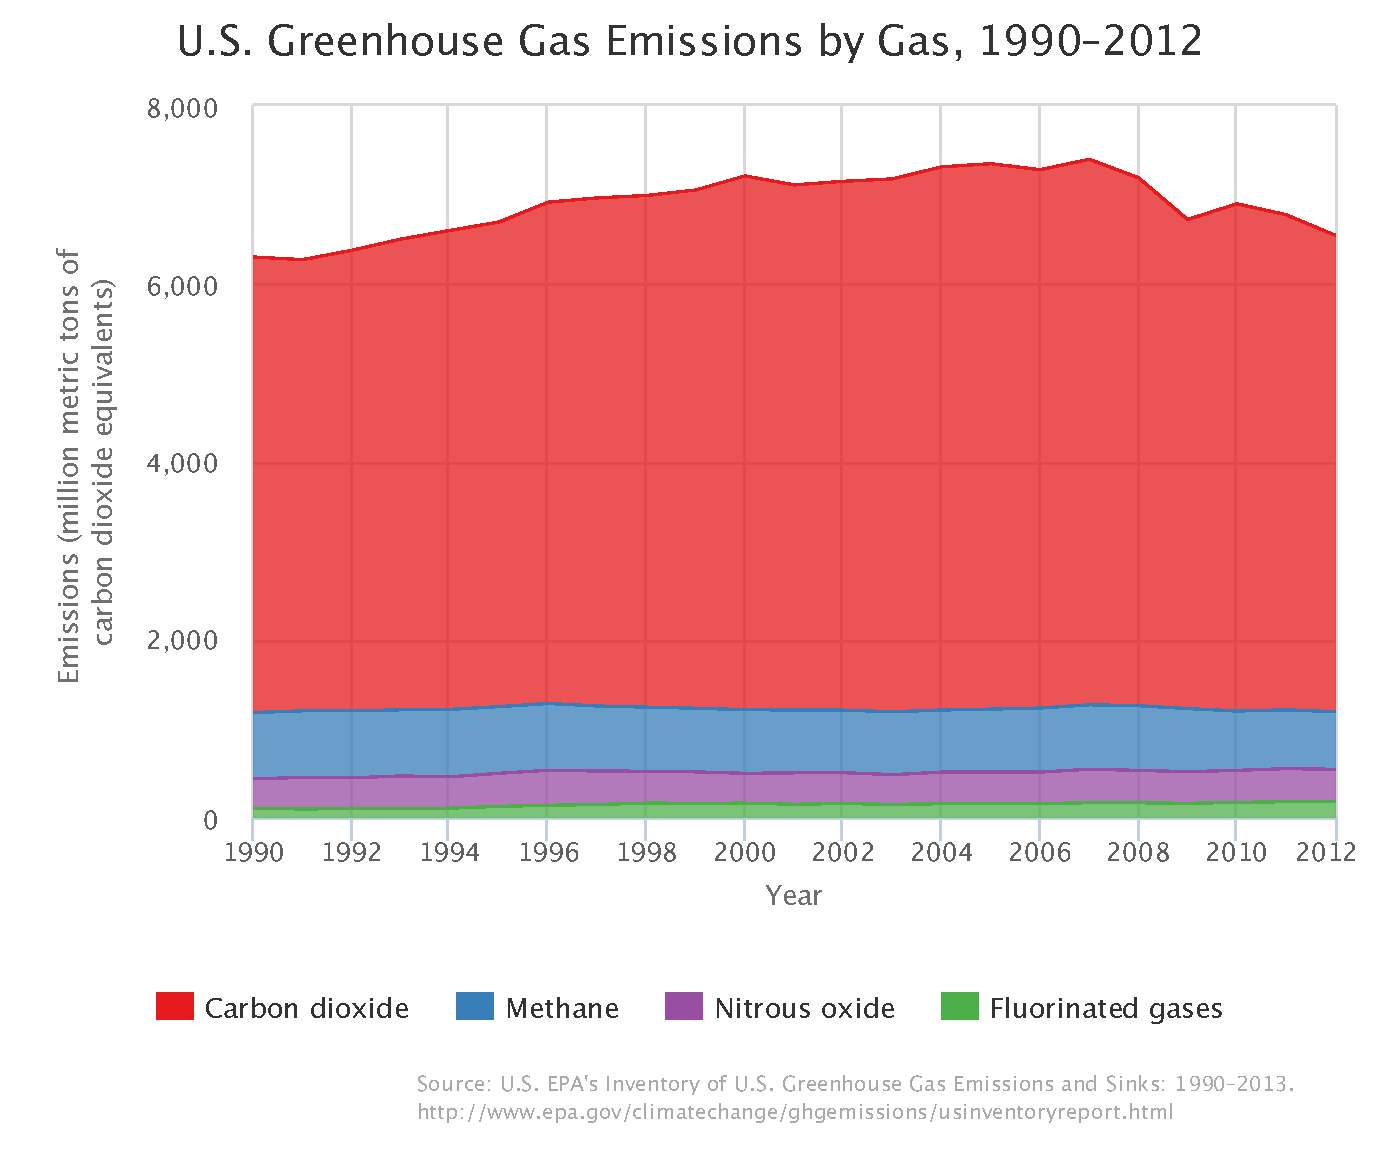
\includegraphics[scale=0.6]{pics/new_d1.pdf}
\caption{GHG Emissions of the USA. (Figure from \cite{debbie}{newfigsepa})}
\label{d1}
\end{center}
\end{figure}

\begin{figure}
\begin{center}
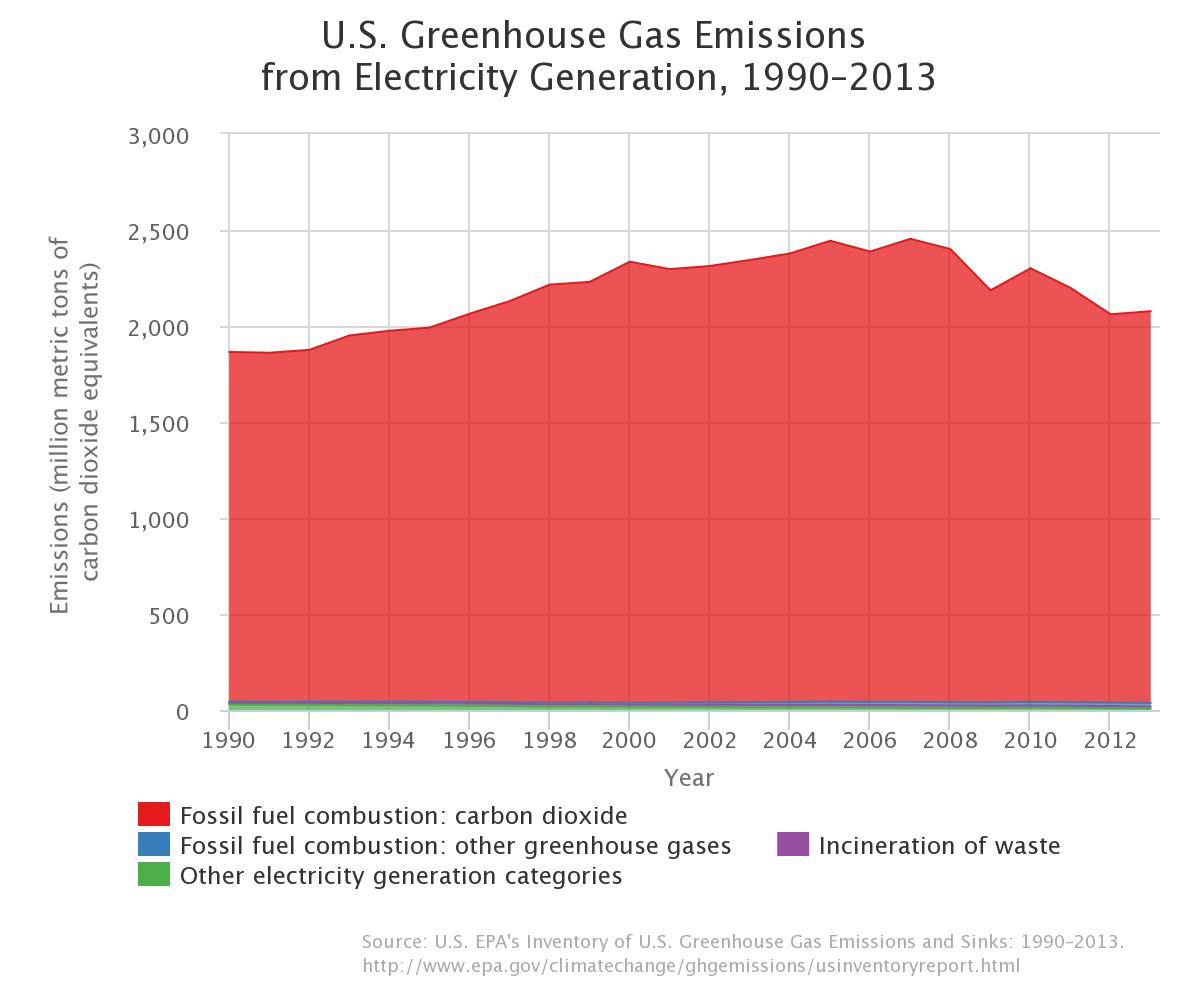
\includegraphics[scale=0.35]{pics/chart.png}
\caption{GHG Emissions due to Electricity of the USA. (Figure from \cite{debbie}{newfigsepa2})}
\label{d1}
\end{center}
\end{figure}

\begin{figure}
\begin{center}
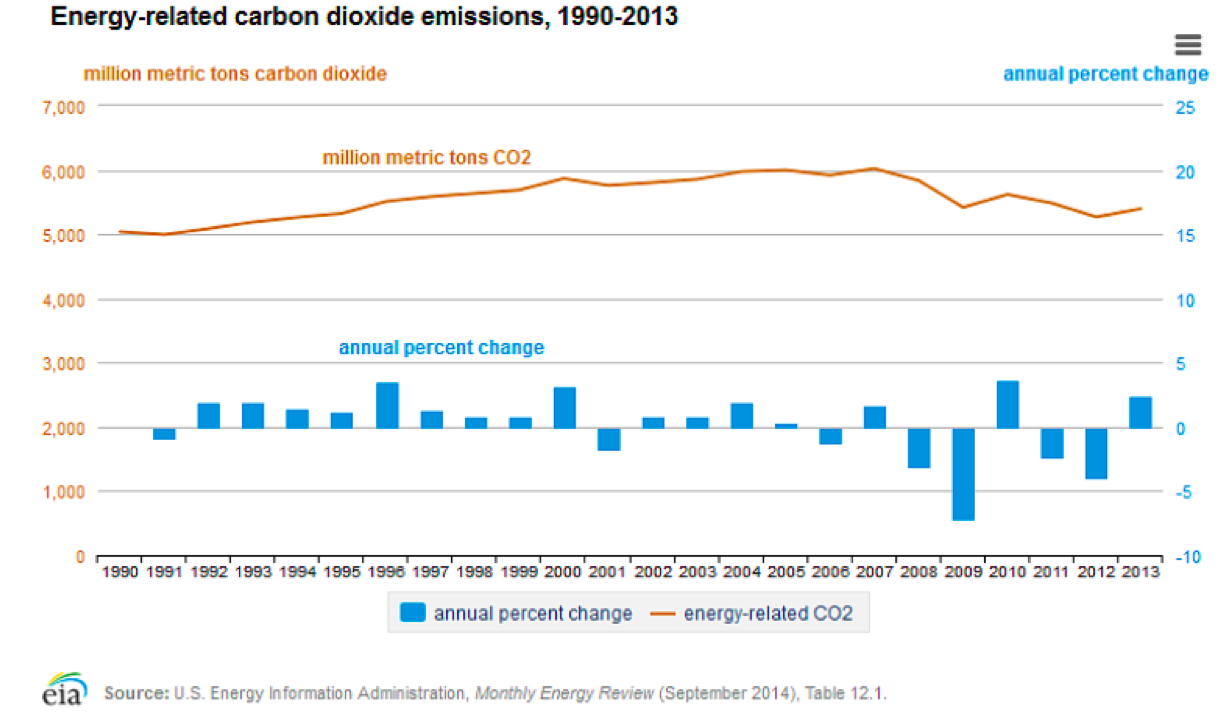
\includegraphics[scale=0.3]{pics/d2.png}
\caption{CO$_{2}$ emissions and annual percent change of CO$_{2}$ emissions of the USA. (Figure from \cite{debbie}{2})}
\label{d2}
\end{center}
\end{figure}

\subsection{Addressing Existing Government Initiatives}
In this section, we highlight how our policy addresses goals within existing government policies.

\paragraph{Executive Order 13514 - Federal Leadership in Environmental, Energy, and Economic Performance} 
\mbox{  }\\
On 5 October 2009, President Obama released Executive Order 13514: Federal Leadership in Environmental, Energy and Economic Performance \cite{debbie}{2}. The purpose of this order was to promote clean and sustainable energy, and that the Federal government should lead by example through improving their energy efficiency, lowering their GHG emissions and measuring and openly reporting their progress towards these goals.
\\\\
\noindent Implementation of our policy would address several of the specific instructions given in this executive order. Section 2(b)(i) of this order directs Federal agencies to consider achieving GHG reductions by \textit{``pursuing opportunities with vendors and contractors to address and incorporate incentives to reduce greenhouse gas emissions...''} \cite{debbie}{2}. Our policy recommendation provides a means to address this by choosing vendors producing the most energy efficient and carbon efficient solar panels to install their panels on the roofs of Federal buildings.
\\\\
\noindent Our policy also addresses Section 2(g)(i) of the Executive Order, which stipulates that \textit{``beginning in 2020 and thereafter, ensuring that all new Federal buildings that enter the planning process are designed to achieve zero net-energy by 2030''}. Installing efficient solar panel on the roofs of Federal buildings will contribute to them being energy neutral. Similarly, our policy addresses Section 2(a)(ii), which involves \textit{``increasing agency use of renewable energy and implementing renewable energy generation projects on agency property ''} \cite{debbie}{2}.
\\\\
\noindent In response to Executive Order 13514, the GreenGov Initiative was launched \cite{debbie}{7}. This initiative called upon all government employees to share ideas about how the goals set out in the Executive Order could be achieved. The top voted ideas were summarized in a report which was released in February 2010 \cite{debbie}{8}. In this report, one of the top-voted ideas by government employees was the installation of solar panels on government buildings.

\paragraph{President Obama's Climate Action Plan} \mbox{ }\\
In June 2013, President Obama’s Climate Action Plan was released. The three main ``pillars'' of this plan were: 1) cutting carbon emissions, 2) preparing for the impacts of climate change, and 3) leading international efforts to against climate change \cite{debbie}{9, 10, 11}. Our policy directly addresses two of the goals in this Climate Action Plan, namely the goal aiming to double the amount of wind and solar energy produced in the USA by the year 2020, and the second aiming to have 20\% of the Federal Government’s energy demands coming from renewable sources \cite{debbie}{11}.

\paragraph{Executive Order 13693 - Planning for Federal Sustainability in the Next Decade} \mbox{ }\\
Very recently, on 19 March 2015, Executive Order 13693 was issued
\cite{debbie}{12}. This Executive Order included very specific goals for GHG emission reduction. Section 3(c) stipulated that 10\% of electricity usage by Federal Agencies had to be generated from renewable sources by 2016, 15\% by 2018, 20\% by 2020, 25\% by 2022 and 30\% by 2025 \cite{debbie}{12}. Section 3(d)(i) stated that Government Agencies should attempt to reach these goals by installing renewable energy sources on site at the Federal facilities \cite{debbie}{12}. These orders would be directly addressed through the implementation of our policy.

\subsection{GHG Emissions from PV Cells}
PV cells do not, that we know of, produce any GHGs specifically by making electricity, however, GHG’s are produced during activities at all stages of the PV cell’s lifetime \cite{debbie}{13}. The analysis of the GHG’s produced throughout the whole lifetime of the PVC, from resource acquisition and manufacture to decommissioning and disposal, is known as Life Cycle Analysis (LCA). The main steps in the lifecycle of a PVC, as well as the approximate percentage of GHG emission at each stage are shown in Figure \ref{d3} \cite{debbie}{14}.
\\\\
\noindent A literature study was performed, aggregating the results of many LCA analyses of PVCs. The resulting lifecycle carbon intensities of the PVCs (measured in grams CO$_{2}$equiv/kWh) had a very broad range, as seen in Figure \ref{d4} \cite{debbie}{13}. However, even with this large range, the GHG emissions from PVCs are still significantly lower than that of coal (Figure \ref{d5} \cite{debbie}{15}).

\begin{figure}
\begin{center}
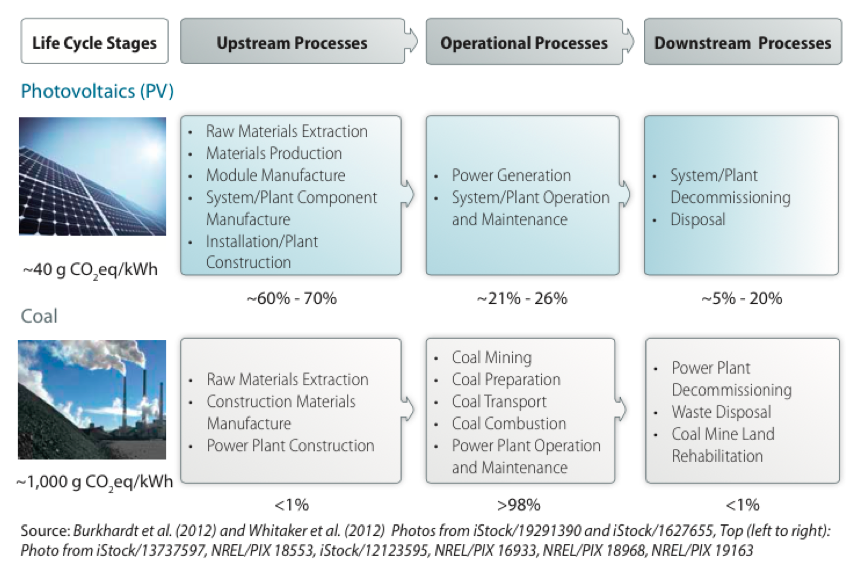
\includegraphics[scale=0.4]{pics/d3.png}
\caption{Stages in LCA of PVCs, and the relative contribution of each stage to the total GHG emissions of PVCs. (Figure from \cite{debbie}{14})}
\label{d3}
\end{center}
\end{figure}

\begin{figure}
\begin{center}
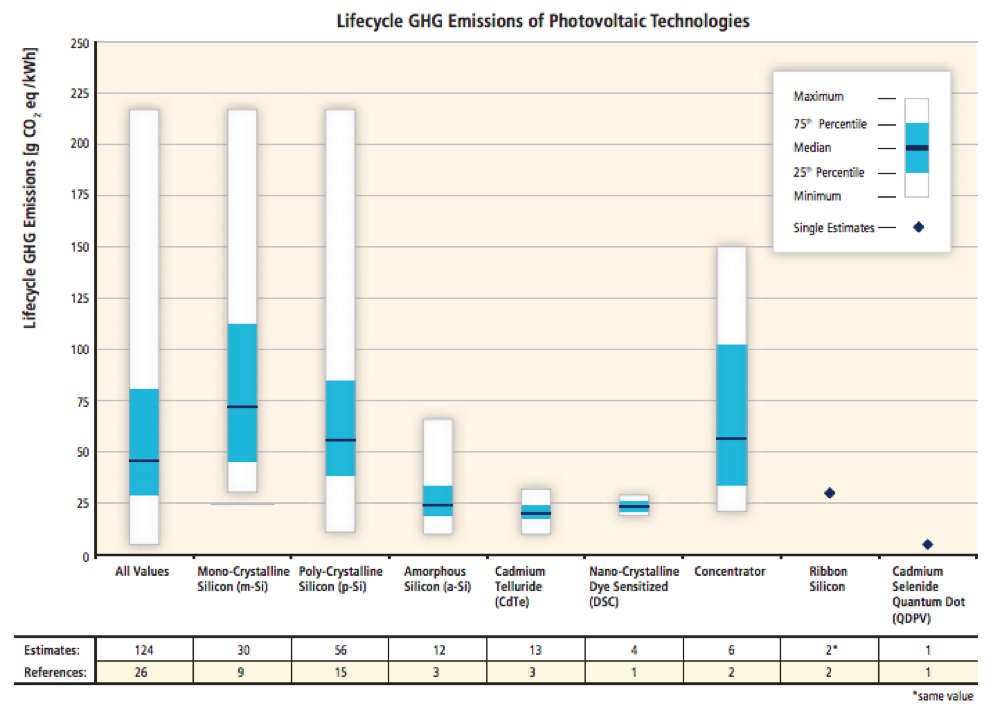
\includegraphics[scale=0.35]{pics/d4.png}
\caption{LCA GHG emissions from different PV technologies. (Figure from \cite{debbie}{13})}
\label{d4}
\end{center}
\end{figure}

\begin{figure}
\begin{center}
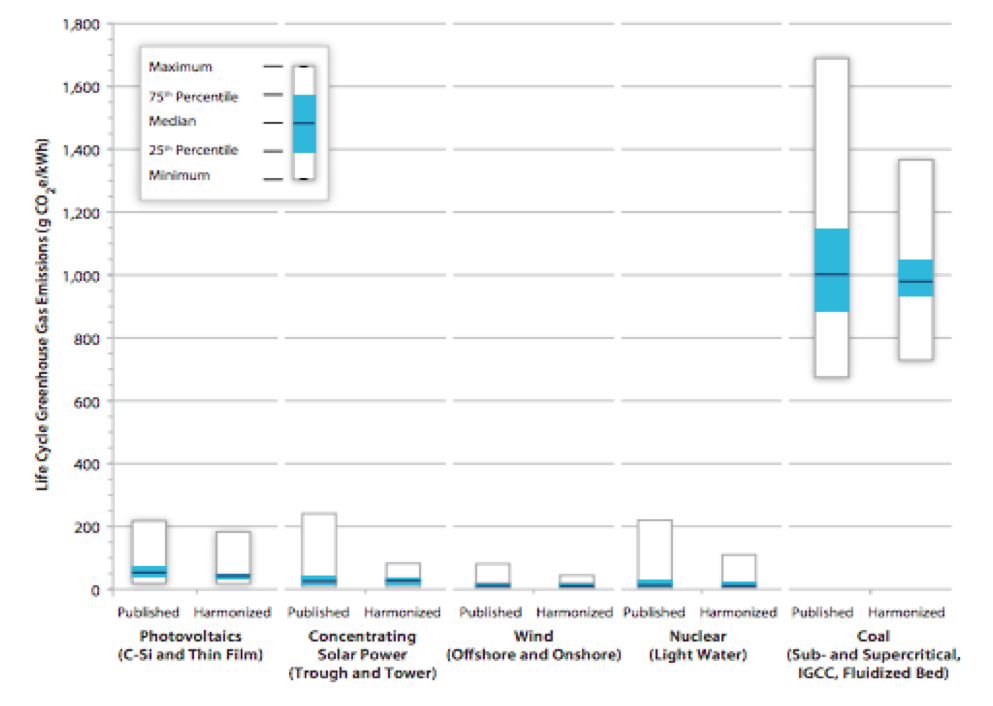
\includegraphics[scale=0.35]{pics/d5.png}
\caption{LCA GHG emissions from different energy sources. (Figure from \cite{debbie}{15})}
\label{d5}
\end{center}
\end{figure}

\subsection{Carbon Emission Analysis}
We performed a Carbon Emissions analysis to attempt to estimate the effect this policy could potentially have on Federal carbon emissions. The Federal Government consists of more than 360,000 buildings \cite{debbie}{7}. As a sample for this analysis, all documented U.S. General Services Administration (GSA) buildings were used.

\begin{table}
\begin{center}
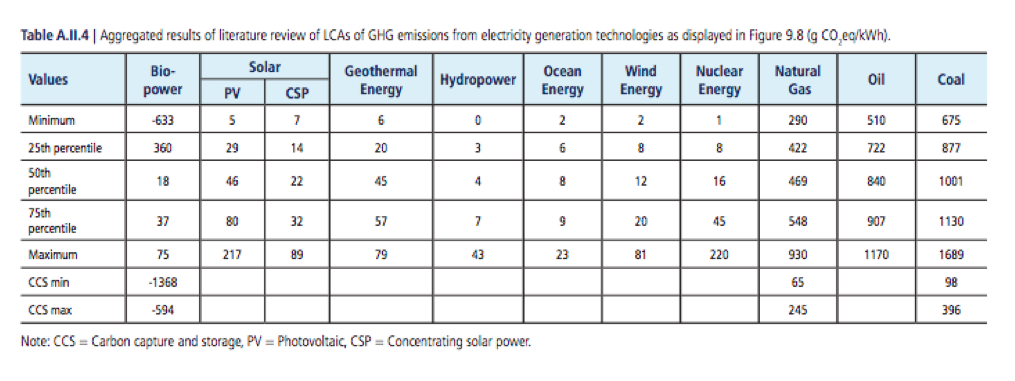
\includegraphics[scale=0.43]{pics/t1.png}
\caption{Solar LCA GHG Emissions. (Table from \cite{debbie}{13})}
\label{t1}
\end{center}
\end{table}

\paragraph{Resources for Carbon Analysis} \mbox{ }\\
A database of all GSA Federal buildings was compiled which also included an estimate of solar insolence at each building, electricity demand of each building, rooftop area and solar energy potential (Compiled by Roison Langan using \cite{debbie}{roisin}). The carbon intensity (mass of carbon dioxide produced per unit energy) for each state was obtained from an energy report published by the U.S. Energy Information Administration (EIA) in August 2014 \cite{debbie}{16}. There was no data available on GHG intensity (mass of all greenhouse gases produced per kWh) at a state-level resolution. A report by the Intergovernmental Panel on Climate Change reported agglomerated GHG emission from various LCA studies of PV panels \cite{debbie}{13}. The values given by this study are in grams CO$_{2}$ equivalents, and thus theoretically contain gases other than CO$_{2}$, however, it has been noted in various sources \cite{debbie}{17, 18} that in LCA studies of PV cells, the major component of GHG emissions is CO$_{2}$. We thus justify using these GHG intensity figures (grams CO$_{2}$ equiv/kWh) as an approximation of the carbon intensity (grams CO2/kWh).

\paragraph{Carbon Analysis Methods} \mbox{ }\\
For each Federal building $B$, the solar potential $P_{{\mbox{solar}}_{B}}$ (kWh/day) was defined as the maximum amount of solar energy which could be produced by the building through rooftop solar panels. This was calculated as:

\begin{equation}
P_{{\mbox{solar}}_{B}} = I \times A_{r} \times \eta
\end{equation}

\noindent where $I$ is the solar insolence at that building in kWh/m$^{2}$/day, (estimated from the average solar insolence of the nearest zip code where possible, or as the state average insolence where no zip code insolence data is available), $A_{r}$ is the estimated rooftop area and $\eta$ is the efficiency of the solar panel, assumed for this analysis to be 16\%.
\\\\
\noindent The carbon emissions by the solar panels $E_{{\mbox{solar}}_{B}}$ in grams CO$_{2}$/day for each building $B$ was calculated as:

\begin{equation}
E_{{\mbox{solar}}_{B}} = P_{{\mbox{solar}}_{B}} \times C_{\mbox{solar}}
\end{equation}

\noindent where $C_{\mbox{solar}}$ is the carbon intensity in grams CO$_{2}$/kWh estimated from Table \ref{t1} \cite{debbie}{13}. This calculation was performed using various $C_{\mbox{solar}}$ values within the spectrum, including the minimum, median and maximum values from Table \ref{t1} \cite{debbie}{13}.
\\\\
\noindent Assuming no solar panels installed, the 'control' carbon emissions $E_{{\mbox{no solar}}_{B}}$ of each building $B$, was calculated as:

\begin{equation}
E_{{\mbox{no solar}}_{B}} = D_{B} \times C_{\mbox{state}}
\end{equation}

\noindent where $D_{B}$ (kWh/day) is the electricity demand of building $B$ and $C_{\mbox{state}}$ is the average energy carbon intensity of the state, measured in grams CO$_{2}$/kWh \cite{debbie}{16}.
\\\\
\noindent The amount of carbon emissions saved $C_{{\mbox{saved}}_{B}}$ (grams CO$_{2}$/day) for a building $B$ through obtaining the maximum amount of its daily electricity demand from rooftop solar panels was calculated as:

\begin{equation}
C_{{\mbox{saved}}_{B}} = E_{{\mbox{no solar}}_{B}} - \left(E_{{\mbox{solar}}_{B}} + \left( \left( D_{B} - P_{{\mbox{solar}}_{B}}\right) \times C_{\mbox{state}}\right) \right)
\end{equation}

\noindent The total percent carbon savings $C_{\mbox{\% saved}}$  was calculated as:

\begin{equation}
C_{\mbox{\% saved}} = \frac{\sum_{B}C_{{\mbox{saved}}_{B}}}{\sum_{B}E_{{\mbox{no solar}}_{B}}} \times 100
\end{equation}

\noindent In order to determine the maximum carbon intensity that a PV panel could have while still
improving the overall carbon emissions of the buildings, the above calculations were performed using all Natural Number carbon intensities between the minimum of 5 grams CO$_{2}$/kWh to the maximum of 217 grams CO$_{2}$/kWh.
\\\\
\noindent The above calculations of $C_{\mbox{\% saved}}$ were also repeated while varying the carbon intensity and the efficiency of the PV cells simultaneously, in order to construct a heatmap of the $C_{\mbox{\% saved}}$ landscape.
\\\\
\noindent 
The results of the carbon analysis are in the supplementary file titled \texttt{carbon\_emissions\_analysis\_DA\_Weighill.xlsx}. The Perl Scripts written to perform these computations are supplementary files \texttt{carbon\_analysis.plx} and \texttt{heatmap.plx}.

\paragraph{Results of the Carbon Analysis} \mbox{ }\\
Assuming that PV cells were installed over the full roof area of all GSA Federal buildings, and assuming a PV cell efficiency of 16\% and a median carbon intensity of 46 grams CO$_{2}$/kWh, the total carbon emissions of these buildings could be reduced from 890732 tonnes/year to 845584 tonnes/year - approximately a 5\% decrease.
\\\\
\noindent Figures \ref{d6} and \ref{d7} show the average carbon emission savings per building and the total percent carbon savings respective, when varying the carbon intensity. These Figures clearly illustrate that if the solar panels installed are not carbon efficient, they will worsen the carbon footprints of the buildings. Assuming a solar panel efficiency of 16\%, the maximum carbon intensity they can have without increasing the average building's carbon footprint is 187 grams CO$_{2}$/kWh. However, this statistic will be affected by the solar panel efficiency. The heatmap in Figure \ref{d8} shows the landscape of percent carbon saved when varying solar panel efficiency and carbon intensity, with green representing positive carbon savings, and red representing negative carbon savings. This kind of tool can be used by the Federal government in evaluating a potential PV cell supplier. Given the carbon intensity and efficiency specifications of the PV cell, it can be determined whether or not it would fall in the ``green zone'' and would contribute positively or negative to the carbon footprint of the building.

\begin{figure}
\begin{center}
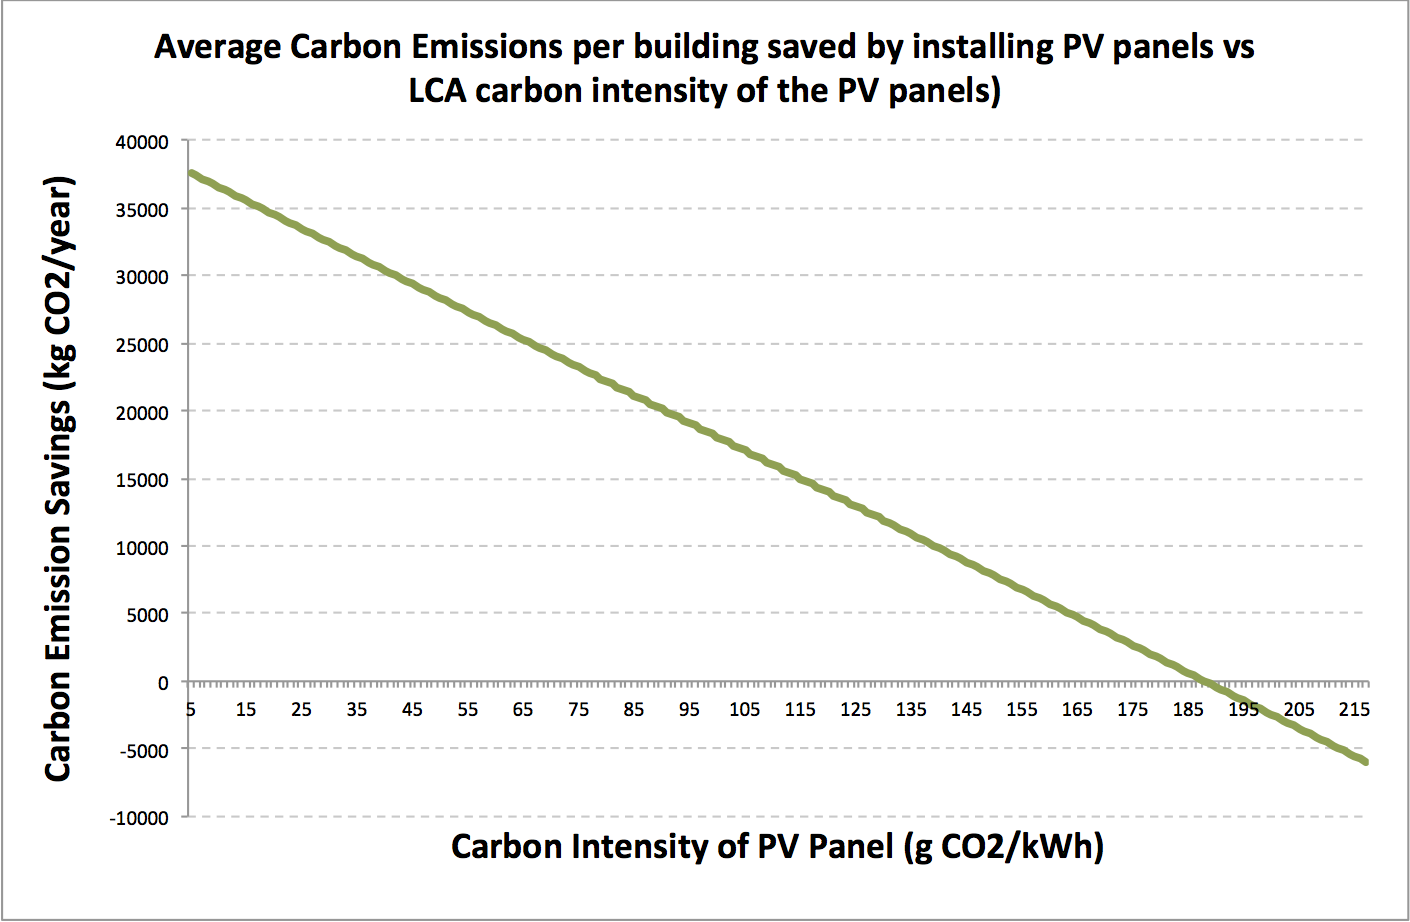
\includegraphics[scale=0.5]{pics/d6.png}
\caption{Average amount of carbon emissions saved vs. carbon intensity of PVCs, assuming a PVC efficiency of 16\% and 100\% of rooftop area utilization.}
\label{d6}
\end{center}
\end{figure}


\begin{figure}
\begin{center}
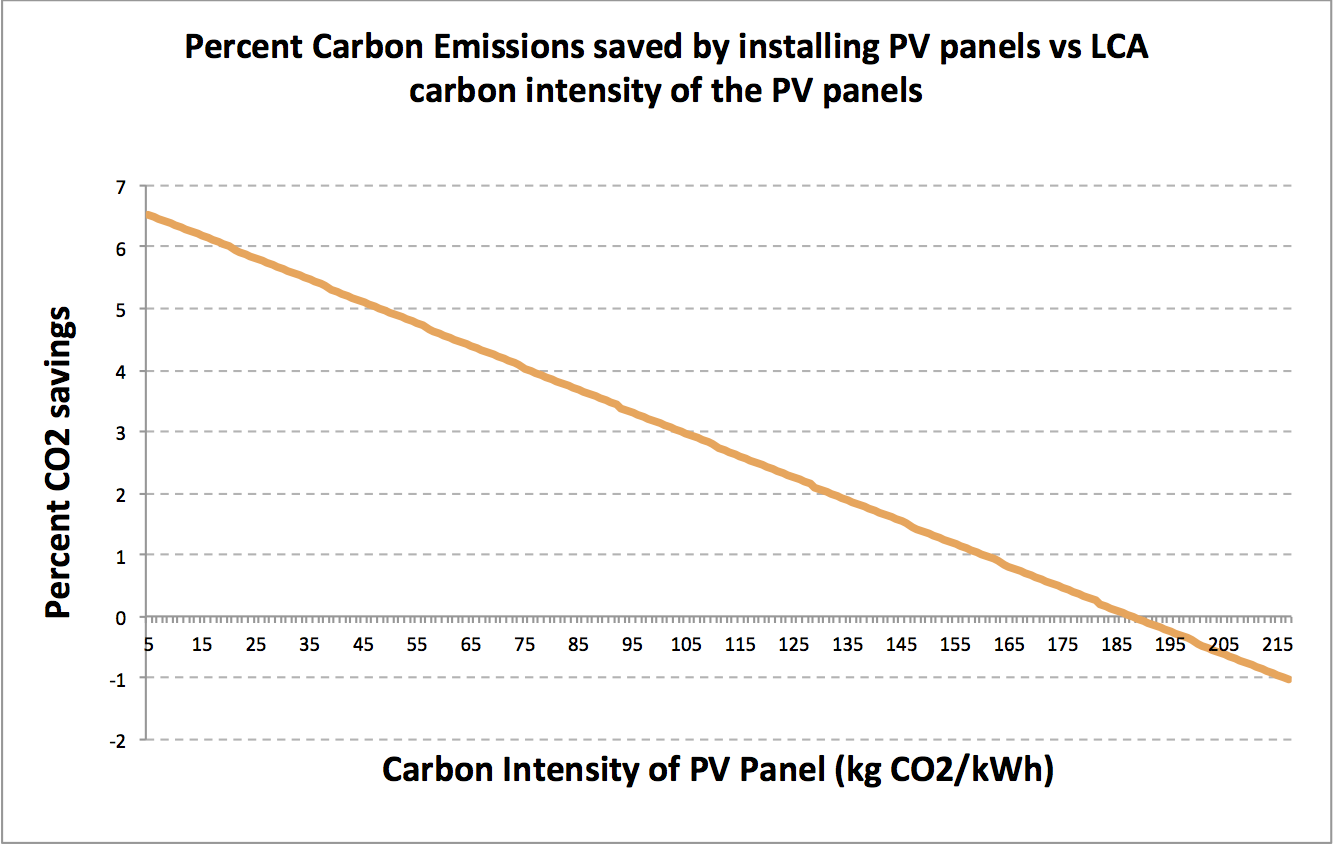
\includegraphics[scale=0.5]{pics/d7.png}
\caption{Percent of carbon emissions saved vs. carbon intensity of PVCs, assuming a PVC efficiency of 16\% and 100\% of rooftop area utilization.}
\label{d7}
\end{center}
\end{figure}


\begin{figure}
\begin{center}
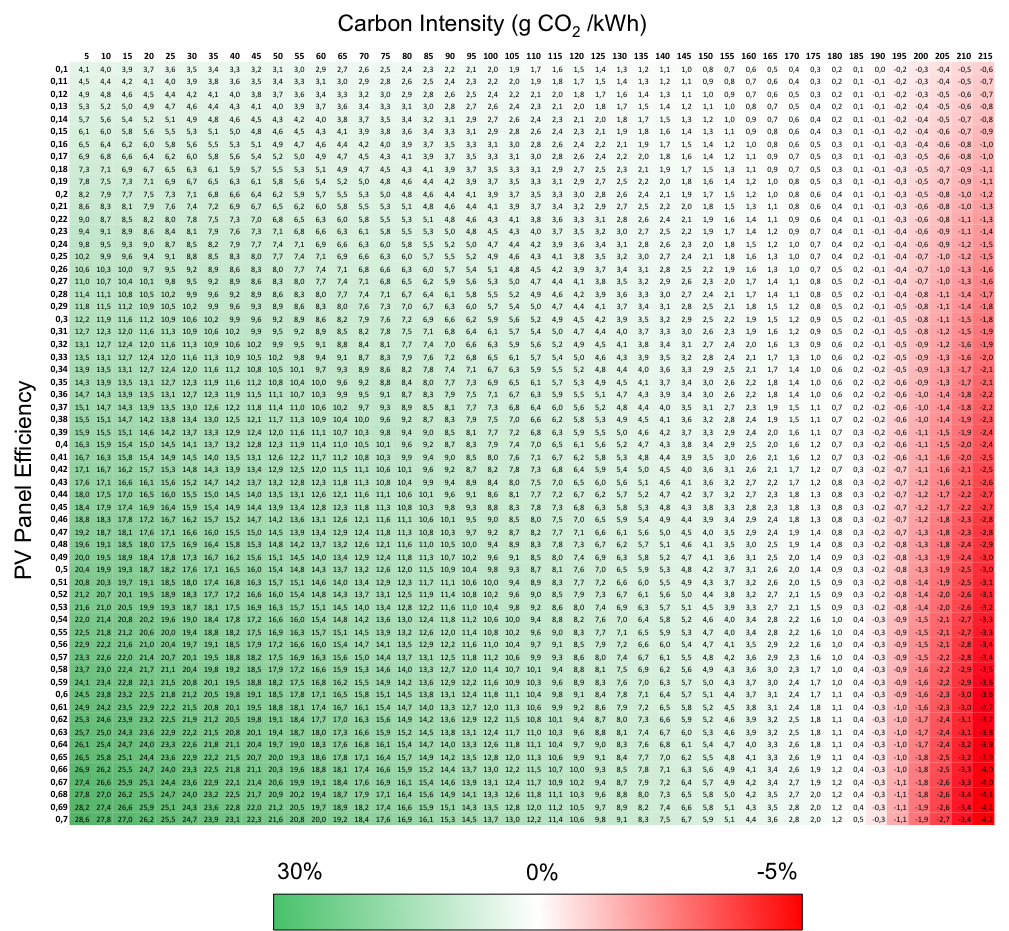
\includegraphics[scale=0.8]{pics/d8.png}
\caption{Heatmap of percent savings while varying carbon intensity (x-axis) and PVC efficiency (y-axis). Green represents positive savings and red represents negative savings.}
\label{d8}
\end{center}
\end{figure}


\subsection{Concluding Remarks}
The implementation of our policy could help address many of the Federal Government’s current goals of lowering its carbon emissions and increasing the fraction of renewable energy consumed by Federal buildings. This will, however, depend on the specifications of the solar panels being produced, in particular, the solar panel efficiency and the carbon intensity. Solar panels will have to be chosen carefully such that they improve carbon emissions and energy efficiency. This, in addition to helping the government meet its energy and emission goals (outlined above) our policy will drive improvement of solar panel efficiency and carbon intensity, and thus drive the market forward.


\bibliographystyle{debbie}{ieeetr}
\bibliography{debbie}{debbie}{References}
\clearpage

% ----- Debbie ----- %
\newbibliography{roisin}
\section{The Potential for Rooftop Photovoltaics}
\par
 If the federal government initiates large-scale deployment of rooftop PVs on federal buildings, the increase in demand would lower the cost of solar PVs. The extent to which federal demand for rooftop solar can effect the PV market hinges on the amount of federal electricity demand which can be met by rooftop photovoltaics. Furthermore, the viability of federal PV rooftop installations the cost and profitability of PV technologies must be considered. This study characterizes the potential energy generation, cost and profitabiliy of rooftop PV for federal buildings.

The energy generated with rooftop PV can vary based on physical parameters including rooftop size, and solar irradiance.  In order to approximate the total solar potential across all federal buildings a detailed dataset of existing federal buildings is required. The GSA provides a digital inventory of all leased and federally owned buildings managed in the United States \cite{roisin}{rtl9}. The federal building inventory includes street addresses, zip codes and gross building area. The approximately 1500 federally owned buildings within the GSA inventory are evaluated for rooftop potential and collectively represent the rooftop potential for federal properties.

\par
To calculate the energy potential of an installed system, the solar insolation on the rooftop surface is computed as function of the solar irradiance, surface area, and exposure time. The amount of solar energy that is converted by the solar panel can then be computed by including the efficiency of the technology and performance ratio of the system. The available solar resource is a key factor for PV energy output and subsequent system profitability. In the US, solar energy varies from North to South, East to West and on smaller scales due to altitude and regional climate. Figure \ref{fig:rtl_pic3}, taken from NREL, shows the variability in solar resources across the country and within state boundaries.  To obtain an accurate approximation of PV rooftop potential, it was critical to utilize the high-resolution values for solar irradiance at each federal building. 

\begin{figure}
  \begin{center}
    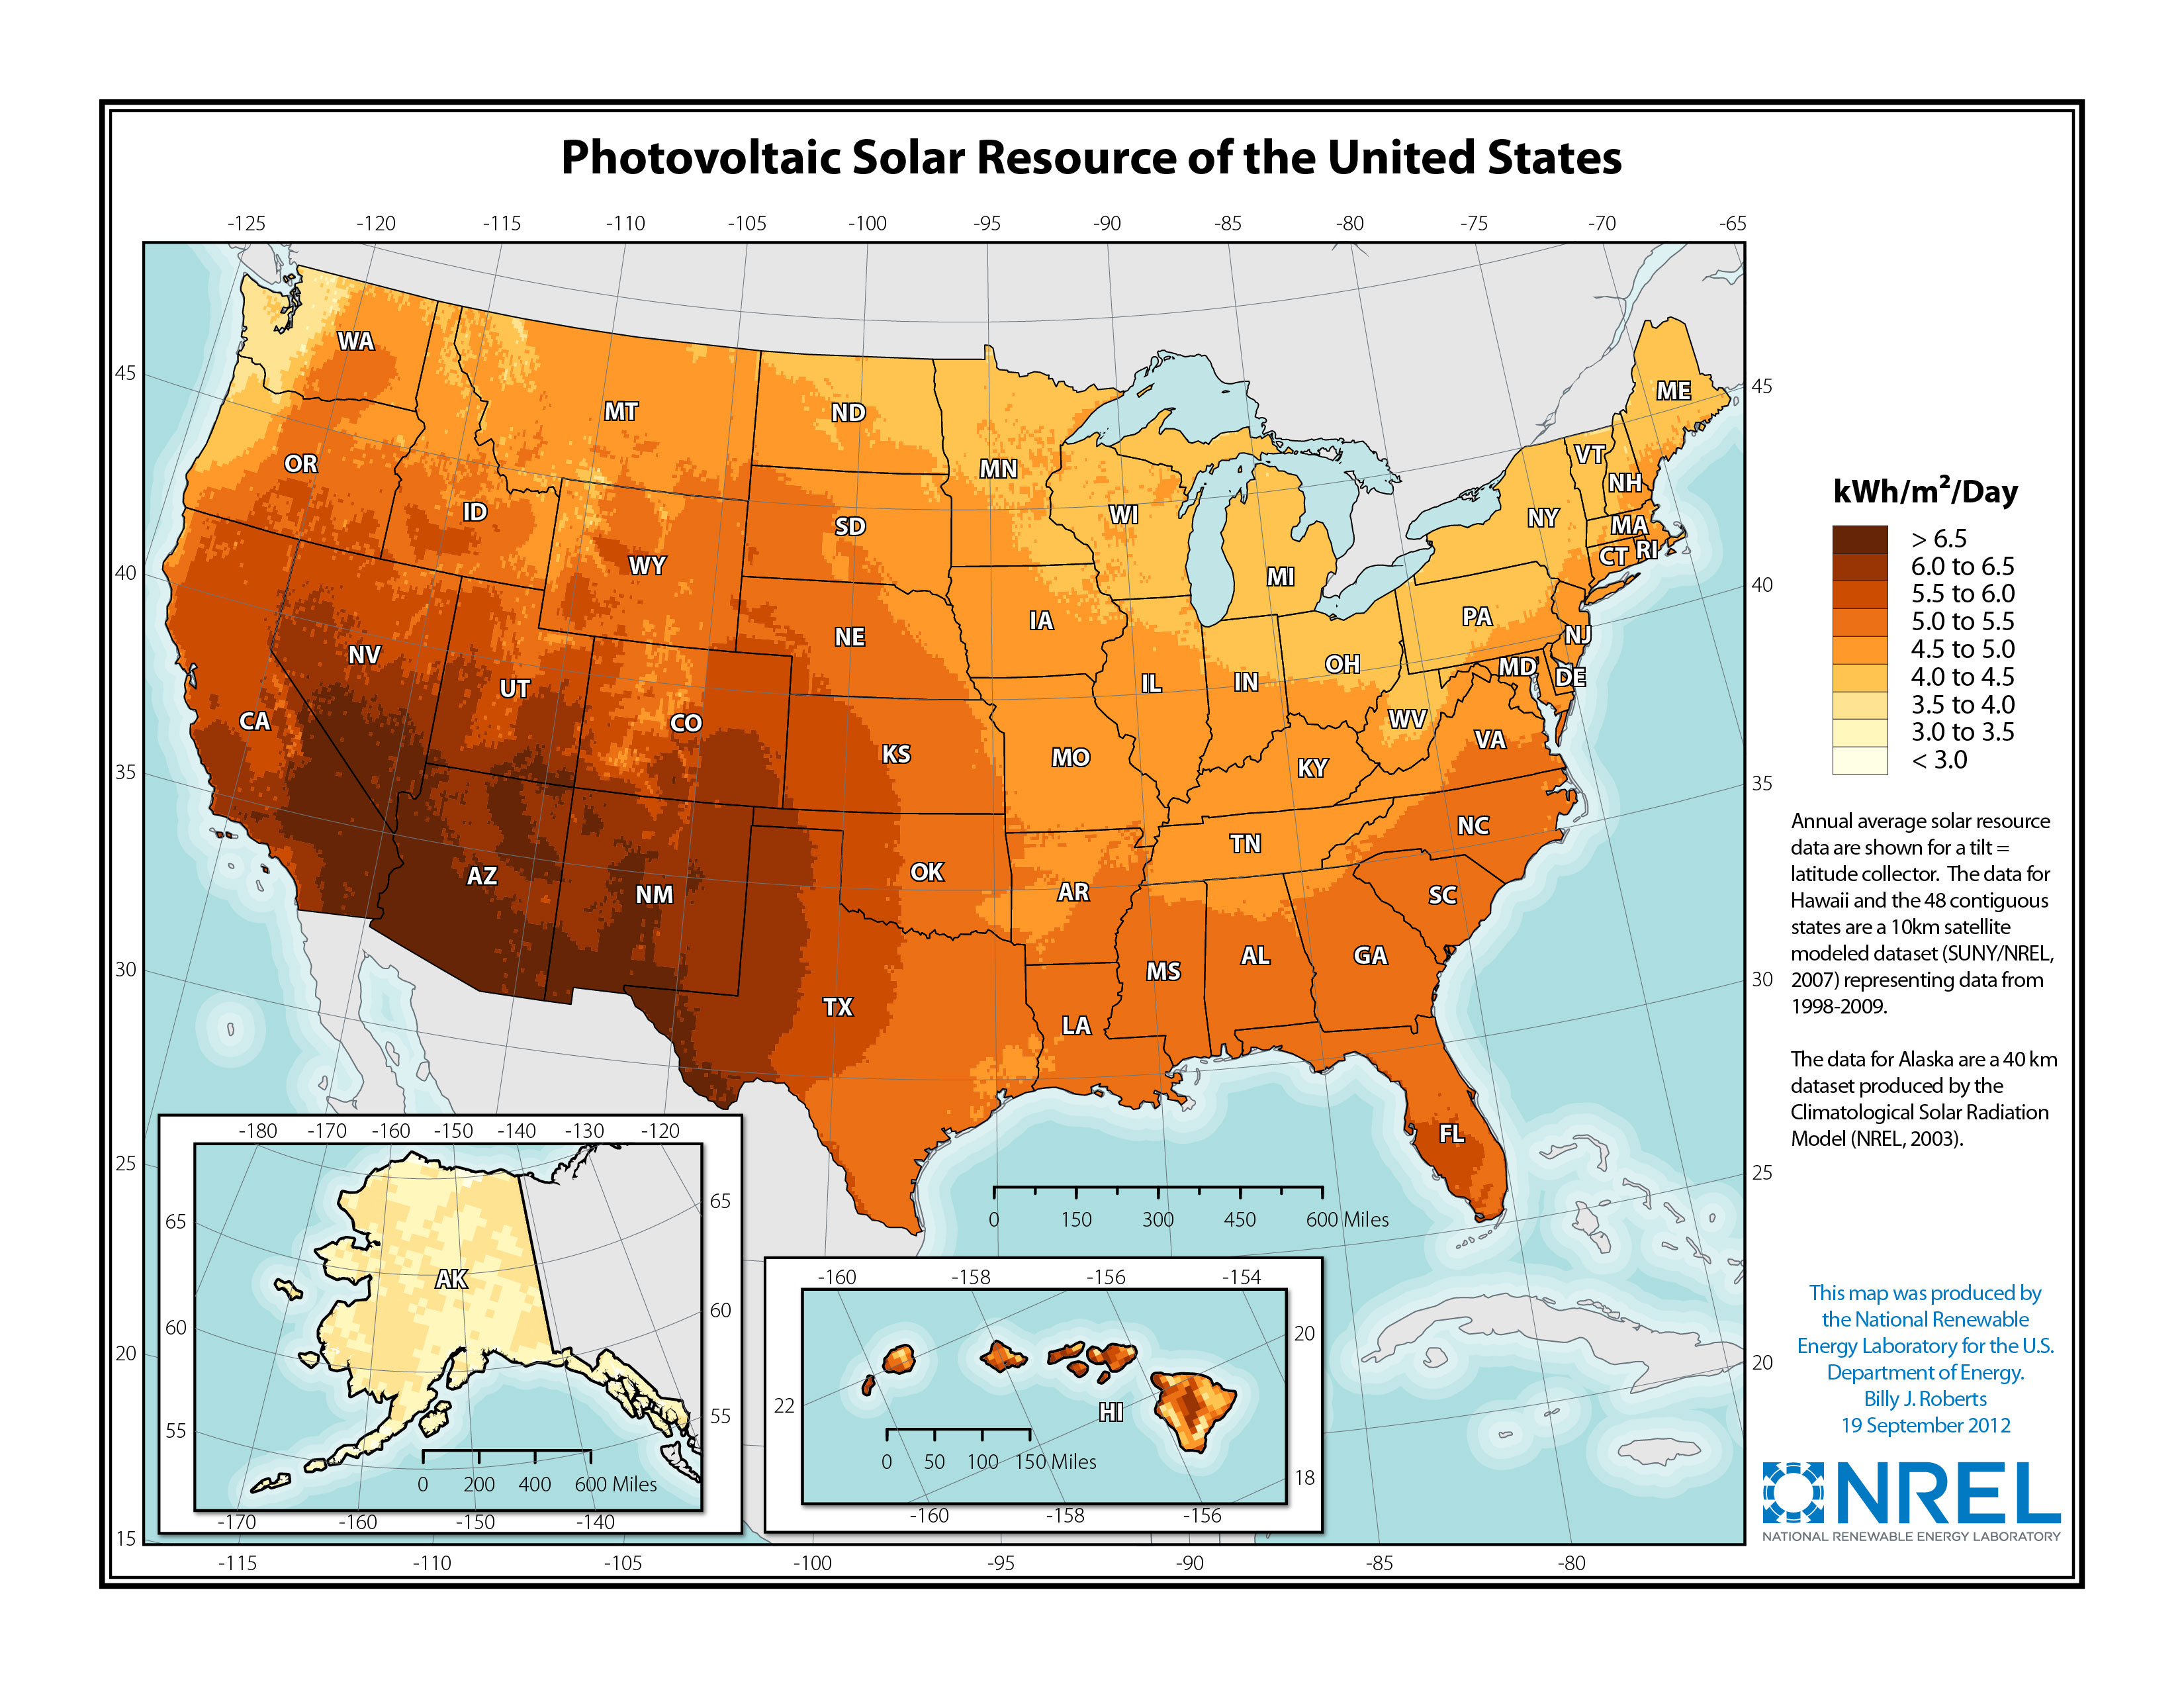
\includegraphics[scale=0.5]{pics/rtl_pic3}
  \end{center}
  \caption{source: NREL}
\label{fig:rtl_pic3}
\end{figure}

The Global Horizontal Irradiance (GHI) for each state and zip code in the US was obtained from NRELs 10-kilometer Solar Data \cite{roisin}{rtl10}. The annual average GHI or total solar radiation, is used determine the solar potential for Flat-pane rooftop PVs at that location. GHI is the sum of the Direct Normal Irradiance (DNI) and Diffuse Horizontal Irradiance (DHI) and ground-reflected radiation.  A procedure known as record linkage, data matching or data merging is used to pair solar insolation values with federal buildings based on their 5-digit zip codes.  In other words, the 5-digit zip code is used to uniquely identify common entries in the GSA building dataset and the 10-kilometer Solar Dataset. For approximately 170 missing GHI values, the state-level GHI value was instead referenced. After matches are made linking GHI values with federal buildings, a new dataset is generated containing both the federal building data and corresponding GHI values. Record matching is implemented in Microsoft Excel using the match and index functions.  The entry matching procedure is also used to obtain state-level electricity rates for each building which is discussed in further sections.  
\par
For a single rooftop PV installation, the energy generated over $N_{days}$ is calculated by:  

\begin{equation}
E_{gen}=A_{eff}*GHI*N_{days}*\eta*P 
\end{equation}

where $E_{gen}$ is the annual electricity production in $kWh$, $A_{eff}$ is the surface area of the solar cells in $m^2$, $GHI$ is the total solar radiation in $kWh/m^{2}/day$, $\eta$ is the PV efficiency, and $P$ is the performance ratio of the solar panels \cite{rtl8}. The effective surface area represents the collective roof area covered by PV panels on a rooftop and is assumed to be 75\% of the roof area. The amount of energy that can be turned into electricity by PVs is effected by the efficiency of the panel, $\eta$, as well as the performance ratio, $P$, a quantity which accounts for losses from dust, inclination, and surface irregularities. 
\par
For each of the 1500 federal buildings, the yearly generation potential of PV modules covering the available rooftop area is computed.  Local GHI values are used in the calculation and rooftop area is approximated from GSA measurements of each of the buildings. The histogram of building gross areas shown in figure \ref{fig:rtl_pic1} reveals most federal buildings to be small, 1 or 2 story structures. 
\begin{figure}
  \begin{center}
    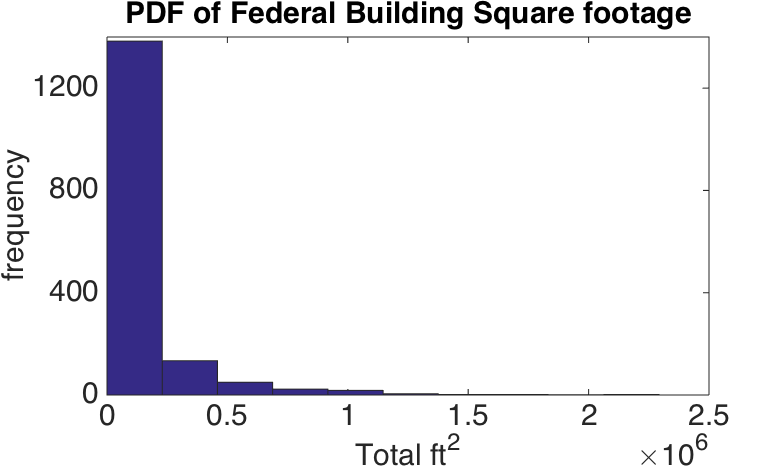
\includegraphics[scale=0.5]{pics/rtl_pic1}
  \end{center}
\label{fig:rtl_pic1}
\end{figure}

For the majority of buildings, the roof area assumed to be equal to building gross area. For buildings greater that 25,000 $ft^2$, it is likely that the building has multiple stories thus a maximium roof area of 25,000 $ft^2$ is used. The upper threshold prevents any severe overestimation of rooftop availability. A performance ratio of 75\% and a PV efficiency of 16\% are assumed to represent the installed solar technology \cite{roisin}{rtl8}. While the yearly generation was computed for each building, the average and total values are supplied in this report. Collectively the 1500 federal buildings are approximated to have 1,636,152 $m^2$ of effective rooftop area which can be harnessed to supply 317,058,200 $kWh/year$ of electricity. The average federal building is found to have an effective rooftop area of 1,073 $m^2$ with which PVs can generate 207,907 $kWh/year$.
\par 

The potential benefit and cost of installing PV on rooftops presents a trade-off between the up-front installation costs and the long-term savings in building energy costs from renewable energy generation. To compute the cost of the system we must consider differences in market PV costs, operation and maintence costs over the systems lifetime and in the different building locations. Due to the lack of data availability on installed PV prices, the most recent cost of commercial rooftop PV is used to evaluate the upfront cost of installation---3,819 dollars per $kW$ \cite{roisin}{rtl4}. Using the cost of installation and the approximated rooftop system capacities ($kW$), the system cost is obtained for each building. 
\par
The electricity rates used to compute the energy savings per building represent the `Average Retail Price of Electricity to Ultimate Customers by End-Use Sector by State' \cite{roisin}{rtl3} and are linked to each building using the 2-letter state acronym and matching procedure outlined above. The yearly savings in building energy costs is computed by multiplying the $kWh$ of PV generation with the market rates of electricity in dollars per $kWh$. To account for the cost of operation and maintence of the system a penalty of .2\% of the upfront capital investment is subtracted from the yearly savings estimate. Finally, the payback period is determined by the ratio of upfront system cost (dollars) over the annual savings (dollars). 
\par
The histogram of the all PV payback periods are shown in Figure \ref{fig:rtl_pic4}. The payback periods for the 1500 buidlings range between 5 and 40 years, with an average of 24 years.
\begin{figure}
  \centering
    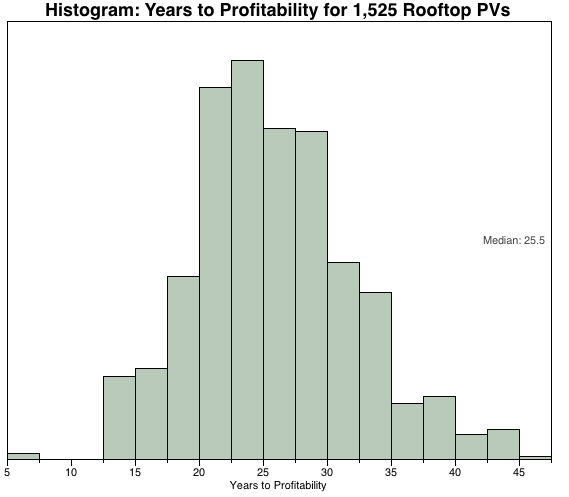
\includegraphics[scale=0.5]{pics/rtl_pic4}
  \label{fig:rtl_pic4}
\end{figure}
 Summary variables of the cost analysis for 2 deployment scenarios are provided in Figure \ref{fig:rtl_pic2}. In each case, the price of electricity is assumed to remain fixed over time. For scenario 1, the cost and profitability calculations are estimated for all 1500 buildings, the average values for a single building and for all buildings are listed in columns 1 and 2 respectively. For the average federal building, rooftop PV installations will breakeven after 24 years and generate 20,220 dollars in energy savings thereafter.  The economic variables are also evaluated for a second scenario in which half of the federally owned buildings are fitted with rooftop solar---those with the shortest profitability timelines. The average and total values for the most profitable half of federal builidings are shown in columns 4 and 5. For the most productive half of federal rooftops, PV installations breakeven on average after 22 years and save 25,137 dollars annualy per building. If PV were installed on half of federal buildings, after 25 years all installations would break even and save 14,957,037 dollars a year for the remaining system lifetime. 

\begin{figure}
  \centering
    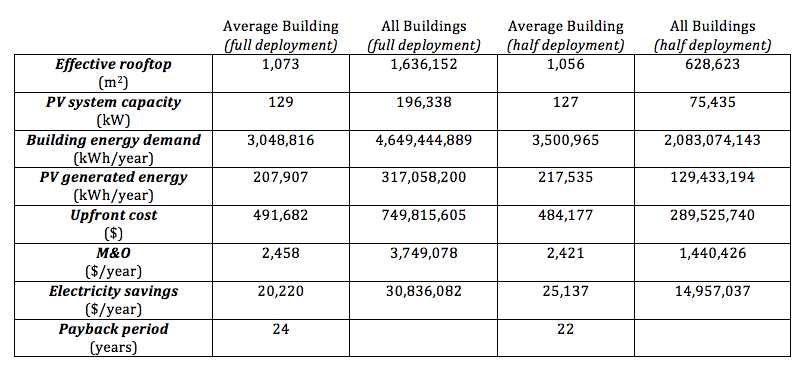
\includegraphics[scale=0.5]{pics/rtl_pic2}
  \caption{Summary of key variables for the full deployment of PV on (1) all federal rooftops and (2) the most profitable half denoted full and half deployment respectively.}
  \label{fig:rtl_pic2}
\end{figure}

By computing the rooftop potential and performing a cost analysis of rooftop PVs for each federal building, we establish a database of economic metrics which can be used to inform the policy deployment and building prioritization. The economic analysis demonstrates that rooftop solar is not only feasible but profitable for the majority of existing federal buildings.

\bibliographystyle{roisin}{ieeetr}
\bibliography{roisin}{roisin}{References}
\clearpage

\chapter{Implementation}

% ----- Julie ----- %
\newbibliography{julie}
\section{Constructing a National Certification Program}

\emph{Julie Cease}

\subsection{Introduction}
The Federal Government currently either owns or leases over 3 billion square feet of building space. A small but expanding number of alternative energy-focused federal facilities has already demonstrated proof of concept in minimizing the federal facility energy consumption footprint. Within the US General Services Administration (GSA), the Office of Federal High-Performance Green Buildings has been authorized by Congress under the Energy Independence and Security Act (EISA) to promote and to expand Federal participation in sustainable property development. Since its inception, the Office of Federal High-Performance Green Buildings has overseen more than 2,500 projects, all certified through the US Green Building Council’s Leadership in Energy and Environmental Design (LEED) program. The purpose of this report is to outline a detailed implementation plan whose objectives are to document a Federal Rooftop Solar Certification Program with strategic emphasis on (1) providing a roadmap for a certification system of national import, and (2) incorporating material criticality concerns where appropriate within the principles of best practice.


\subsection{Developing a Federal Rooftop Solar Certification Program}
Currently, LEED represents the principle system for rating sustainable design measures under the US Green Building Council directive. The Green Building Certification System Review published in March 2012 and prepared by the US Department of Energy (DOE) in accordance with EISA § 433(a) and 426(h) specifies EISA-sanctioned criteria to be used in reviewing certification systems. Specifically, the certification systems must meet three standards both for new construction and for existing buildings; (1) they must employ whole building evaluation, addressing key sustainable design and operations metrics, (2) they must be available in the US market, and (3) they must have third party certification. Whereas the afore mentioned methodology presents screening criteria for green building designs as a whole, the solar photovoltaic mandate proposed here, because it regards rooftop installation alone, will address the last two criteria for determining the minimum system requirements for Federal Building solar photovoltaic installations. The recommendations to follow fall under the EISA rubric and adhere to the EISA criteria.


\subsubsection{Technologies and Feasibility Study}
The first phase of certification will entail a technologies and feasibility study to be conducted by a third-party auditor responsible for performing onsite rooftop and general location-centered evaluation. The Green Building Certification Institute (GBCI) will provide third-party certification. Site and structural assessment as well as all documentation to be submitted in response to site evaluation and verification will be undertaken within the official auspices of the GBCI. For this review, the following considerations will be assessed:

\begin{itemize}
\item Extant Neighborhood
\item Landscape Infrastructure
\item Insolation Potential
\end{itemize}

The purpose of the Technologies and Feasibility Study is to screen proposed and existing properties for both for future optimization and for resultant impracticable obstacles that may interfere with the installation of a solar energy system. The scope of such a study includes an evaluation of the extant neighborhood, which includes the urban block(s) surrounding the proposed site, along with the general landscape geometry, which enables mapping of discrete sky verses shadow segments impinging on future installation infrastructure. The urban block(s) surrounding a proposed site may impose significant influence on solar access. Tall residential and commercial buildings produce shading masks throughout a solar day. Geometric topography of neighboring buildings combined with varied solar heights at local latitudes across the United States will of necessity converge to produce diverse access conditions, all of which will dictate the feasibility of a particular solar photovoltaic installation.
\\\\
\noindent Sustainable building design software offers detailed and highly analytical profiling of either existing or proposed sites from the earliest stages of architectural design. Autodesk Ecotect Analysis is one program that enables multiplexing of disparate data streams into a composite energy picture. Figure \ref{juliefig1} shows an Ecotect analysis example, in which data sets including building typology, lighting simulation, solar insolation, direct shading, and seasonal climate analysis can be combined in an interpolated 3D visualization of the target site.

\begin{figure}
\begin{center}
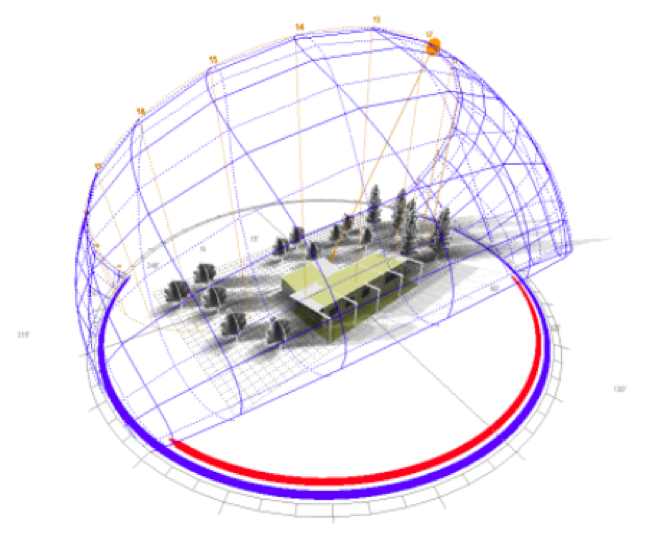
\includegraphics[scale=0.7]{julie_pic_1.png}
\caption{Ecotect analysis example}
\label{juliefig1}
\end{center}
\end{figure}


\subsubsection{Alternatives Evaluation}
The second phase of certification involves an evaluation of alternatives. As with the Technologies and Feasibility Study presented above in Phase One, the Green Building Certification Institute (GBCI) will provide third-party assessment of alternatives. Alternative considerations will include:

\begin{itemize}
\item Financing Options
\item Weathering
\item Module Specification
\end{itemize}

Consistent with a mandate seeking to provide maximum flexibility and adaptability where site-specific implementation is concerned, three financing options come under consideration: cash purchase, power purchase agreement (PPA), and lease. A cash purchase option entails a one-time upfront purchase cost where the purchaser owns the system hardware. Progress payments occur coincident with construction progress. The option to lease a rooftop solar photovoltaic system demands zero or low upfront cost, but requires a recurring lease payment combined with a fixed payment for the system hardware. The PPA represents a versatile option wherein the purchaser incurs no upfront cost but pays a fixed rate for energy in the form of payment per kWh consumed.
\\\\
\noindent Due to incomparable climactic variation across the US, issues of module weatherability arise. Module producers typically guarantee photovoltaic panels for 20 to 25 years, with warranty coverage specifying performance of at least 90\% capacity for the first ten years and at least 80\% capacity for the remaining fifteen years. All photovoltaic module designs must undergo testing in accordance with the International Electrotechnical Commission (IEC) for qualification of design, materials, and defects. Wafer based silicon is certified under IEC 61215 whereas thin film technologies undergo qualification under IEC 61646. Importantly, neither of these qualification regimes subject models to test protocols that include or combine weather exposure testing—even though both formal laboratory and outdoor accelerated weather testing is available.


\paragraph{Evaluating Extreme Service Environments} \mbox{ }\\
Within the continental US, Alaska and Hawaii, three extreme service environments exist: desert/monsoonal, tropical, and polar. Taking data from the Technologies and Feasibility study described above for Phase One, modules targeted for deployment in extreme service environment climatic regions must undergo advanced durability testing prior to certification. Unlike IEC testing, which focuses on design type qualification tests, which are engineered to identify short-term failure, Accelerated Environmental Testing (AET) reproduces likely field conditions using a set of comprehensive climate stresses. Stress testing comprised of multiple simultaneous loads including temperature, humidity, salt spray, extreme UV, freeze-thaw cycling, and maximum power draw produces accumulated damage and field failure representative of long-term outdoor extreme exposure. The weathering testing proposed here is based on a global composite climate standard compiled under the Köppen-Geiger climate classification system. This climate map is used to predict geographic regions situated within worst-case climate boundary conditions.
\\\\
\noindent Alternatives decisions with respect to module selection and orientation can accommodate a wide array of rooftop configurations and site-specific insolation patterns. Solar panel selection, however, will need to come from top tier producers if robustness and efficiency are to be maintained throughout the mandate. Modules produced in the US must comply with competitive best practice dynamics in terms of research and development, material quality, production processing and energy conversion efficiency. Pike Research, a market research firm based in Boulder, Colorado, specializing in providing rigorous technical analysis of global clean technology trends, recently published a tier system whereby global solar photovoltaic module producers achieve a general rank according to in-house versus outsourcing of manufacturing processes, investment in research and development, manufacturer longevity, and stringent quality control. Price to consumer plays no role in the ranking system.

\paragraph{Tier One Module Producers}\mbox{ }\\
Tier 1 solar photovoltaic modules represent panels fabricated from the top 5\% of solar manufacturers. Tier 1 producers control all stages of module manufacture in a vertically integrated production process. Photovoltaic modules, whether based on silicon or thin film technologies, begin component level deposition or build-up in-house and remain in- house through the entire production process—through panel assembly and module framing to installation and warranty. Tier 1 ranked producers invest consistently and comprehensively in research and development. Hence, these module manufacturers often lead the industry in offering state-of-the-art innovation in both process and product. Furthermore, Tier 1 manufacturers employ advanced robotic fabrication techniques with demonstrated correlation to engineering quality. Robotic fabrication not only reflects a low margin of off-specification product due to device defect and failure, it reduces critical material in the industrial waste stream. Lastly, Tier 1 producers must demonstrate longevity in a relatively young industry through viable commercial manufacture of solar photovoltaics for a minimum of 5 years.

\paragraph{Tier Two Module Producers}\mbox{ }\\
Whereas Tier 1 modules typically lead the industry with electrical conversion efficiencies above 21\%, Tier 2 modules operate at competitive efficiencies of 15\% or greater. Tier 2 panels are considered to be within roughly the top 20\% of all modules produced, although the manufacturers represent approximately 8\% of the solar photovoltaic production market share. Producers ranked within Tier 2 typically account for the best small to medium scale manufacturers. These are the producers who fabricate good quality modules, but whose assembly and production processes take place only partially in-house. Tier 2 producers rely primarily on manual labor in addition to robotic assembly and test of cells in production. Even though the grade and type of silicon or the elements in a thin film cells may be identical to those deployed in the manufacture of Tier 1 cells, off-spec modules and semiconductor grade scrap materials will enter the industrial waster stream at a higher rate for Tier 2 fabrication and production lines. Unlike Tier 1 producers, who drive innovation, Tier 2 producers generally invest little in research and development, having typically between 2 to 5 years production experience in photovoltaic manufacture.

\paragraph{Tier Three and Other Module Producers}\mbox{ }\\
Whereas Tier 3 companies comprise the bulk of the manufacturing market, these solar photovoltaic manufacturers employ only limited robotics and no advanced production technologies in their manufacturing operations. By and large, Tier 3 producers simply assemble solar panels. Since these companies neither produce silicon cells nor fabricate thin films in-house but rely nearly exclusively on manual labor to construct modules, quality and durability in their product lines can vary widely. Not only do solar cell components that have been produced by hand lack the consistent and reliable quality control of an automated system, the devices themselves lack the stable and often state- of-the-art efficiency of the Tier 1 and Tier 2 solar panels. A characteristic Tier 3 company has 1 to 2 years of experience assembling solar panels using components that have been manufactured out-of-house. Furthermore, a typical Tier 3 producer invests nothing in research and development and performs assembly and test without the aid of sophisticated quality assurance measures throughout the production process. Only modules produced by US producers in Tier 1 and Tier 2 will be included in the alternatives selection process.

\paragraph{Evaluating System Configuration}\mbox{ }\\
Rooftop solar photovoltaic systems offer attractive sites for module deployment precisely because they take advantage of free building space at close range to pre-existing utility connections. Rooftop area, however, determines the maximum array size of a given solar installation, and in some instances, limits the size of the system to distinct disadvantage. In constrained or limited areas, lightweight ballasted systems can be deployed to marked advantage over conventional rack-mounted systems. At each proposed or extant site, maximizing output at the module level means evaluating available roof area for optimal panel configuration and tilt, depending on latitude.
\\\\
\noindent System configurations may make use of modules that sit horizontally or at a tilt angle. The final size of the system is governed by the ground coverage ratio (GCR), which represents the area covered by photovoltaic modules divided by the total rooftop area occupied by the installation. For each system, tilt angle and GCR alternatives can be chosen to optimize system capacity and energy output at the module level. This strategy maximizes the economic return of the installation by prioritizing the performance of the most expensive component in the system.
\\\\
\noindent As tilt angle increases, however, GCR must of necessity decrease as row spacing widens to avoid inter-row shading. In an effort to achieve the lowest levelized cost of energy at each location, however, the site conditions, module selection, available rooftop area, and climate will all factor into the overall system decisions. For smaller installations, such as Federal Building rooftop systems, a balance must be achieved between optimum tilt angle and economically viable GCR. In a study on the impact of tilt angle on system economics for area constrained rooftops performed for SunPower, a high-efficiency crystalline silicon photovoltaic module producer in the US, buildings with low area installation availability returned the greatest economic surplus at low to moderate tilt angles combined with high GCRs.

\subsubsection{Installation Certification and Permitting}
The final step in a green building rooftop solar installation certification program is permitting. Permits are required for the installation of all building-connected solar energy systems. Currently, the GSA evaluates green building certification systems as required under § 436(h) of the EISA. Every five years the GSA assesses certification levels regarded as being “most likely to encourage a comprehensive and environmentally sound approach to green buildings.” The GSA’s findings are submitted to the Secretary of Energy who, in consultation with the Department of Defense (DOD) and GSA leadership, determine the system(s) to be adopted across the Federal Government. The certification guidelines proposed here would be incorporated into the US Green Building Council’s LEED v4 2014, last reviewed in 2014.
\\\\
\noindent The certification guidelines recommended in this report take their lead from the evolution of successful certification systems for green buildings currently prescribed by the US Green Building Council and underway on the national market. In like manner, the certification process described here, which applies to all existing Federal Buildings, in addition to those proposed as new construction and those under consideration for major renovation, seeks to provide robust criteria for high-performance solar photovoltaic energy installations. As such, the requirements for feasibility and evaluation are driven by the following Federal green building requirements:
\begin{itemize}
\item Energy Independence and Security Act (42 USC Part 152) EISA
\item Energy Policy Act of 2005 (Public Law 109-58) EPA
\item Strengthening Federal Environmental, Energy, and Transportation Management (Executive Order 13423, 2007, codified by 111th Congress, HR1105 § 748)
\item Federal Leadership in Environmental, Energy, and Economic Performance (Executive Order 13514, 2009)
\item Federal Leadership in High Performance and Sustainable Buildings Memorandum of Understanding (signed by 21 Federal agencies January 2006) and Guidance (approved by the Office of Management and Budget December 2008)
\end{itemize}

\noindent The purpose of installation permitting is to outline the specific findings that must be made and documented prior to construction. Whereas local governments may have state or local building codes or local ordinances regarding land use and building standards, the national certification program will ensure that where solar energy is generated for on-site use, the national mandate will take precedence over local governments’ ability to unreasonably prohibit or restrict rooftop solar installations.
In addition, installations must meet design requirements under all applicable laws and codes. Certification permitting applications must be submitted by the applicants of record, who will include a Registered Architect and a Professional Engineer. The filing professionals must make all necessary technical certifications, perform all structural, electrical, and safety assessments. Projects submitted for permitting may be filed as part of a new building or as an alteration permit application. Each of these areas is discussed in detail in the sections to follow.

\paragraph{Structural Requirements}\mbox{ }\\
For new construction, additional loads imposed by solar photovoltaic systems can usually be addressed by means of a straightforward and inexpensive approach. Where rooftop retrofitting is required, however, installation of a solar system adds weight to a rooftop design that must be accounted for to ensure that the building can safely bear the additional weight. Solar rooftop installations represent static or a “dead” loads, but the cost and complexity involved in retrofitting will vary according to the existing structure and specifications of the building and the roof.
\\\\
\noindent Although an installed solar photovoltaic system represents a static load under most conditions, solar panels have the potential to impose far greater dynamic load profiles under seismic forces, snow accumulation and wind forces. The assumed design loads for existing buildings, which have already taken into account the required size and spacing of support for a roof given covering type, roof slope, and if appropriate snow loading, must take these potential dynamic loads into consideration. Generally, the structural support required for a generic roof does not include photovoltaic systems.
\\\\
\noindent Additionally, the rooftop must be inspected prior to installation to verify and document any rooftop obstructions that are not shown on the original plans. Existing roof construction must be verified and all potential framing connections identified. The construction inspection must reveal that the panels will not be installed on non- permitted structures such as roof extensions, and that the panels or their framing will not impede roof drains, down spouts, plumbing or HVAC vents. A professional structural engineer or a licensed and registered architect must verify the proposed plans prior to construction of the solar photovoltaic rooftop installation as part of the permitting process.

\paragraph{Electrical Requirements}\mbox{ }\\
All proposed rooftop solar photovoltaic installations must be approved and/or designed by a professional electrical engineer. Individual system components must be identified and listed as compliant with the application for proposed use to ensure a code-compliant system. This applies to all solar photovoltaic system components including but not limited to the installation’s panel types, the modules, inverters, connectors and disconnects. All equipment must be identified and listed for each application to include UL 1703 listing for modules and UL 1741 for inverters and charge controllers. AC modules must present appropriate markings, have overcurrent protection, disconnects and ground fault protection.
\\\\
\noindent The construction inspection must confirm that the installed solar electric system substantially conforms to the architecturally approved plans. This includes verification that the solar electric generating system installation includes no other equipment or components other than those identified and listed as compliant. The solar generating system must not include components or subcomponents of a non-solar electric generating system. Finally, the location of electric disconnects, meters and inverter boxes must be identified. The locations of such components must match the locations shown on the proposed plans.
\\\\
\noindent Prior to final approval, all conductors and wiring methods must be verified to ensure that standard building wire conductors and wiring methods will be employed. All conductors must be rated for service conditions. Photovoltaic source and output circuit conductors to operate in excess of 30 V must be installed in readily accessible locations. Moreover, photovoltaic source circuit wiring conductors must have 90 0C sunlight and wet service resistance. Only single conductor type USE-2 and specifically listed and labeled as photovoltaic wire will be permitted for these circuits. Polarized, non-interchangeable, guarded and locking connectors must be employed that have first-to-make/last-to-break contact for all grounded conductors.

\paragraph{Overcurrent and Array Ground-Fault Protection}
In addition to conductors, all photovoltaic output and inverter output circuits must be provided overcurrent protection rated no less than 125\% of current maximum. Likewise, transformer overcurrent protection must be provided and verified prior to permitting. Overcurrent protection must also be listed for each required device with appropriate voltage, current and interrupt ratings documented. Disconnects must be provided to isolate inverters and charge controllers from all underground conductors. The disconnects provided must function independently by means of disconnect fuses. These fault isolation circuits must disconnect from all power sources when a fuse is energized from any circuit direction. Disconnects must open all underground conductors, be readily accessible and externally operated.
\\\\
\noindent  Array disconnects between the photovoltaic power system output and all other building conductors must be provided and installed at readily accessible locations. These sites may be on the outside of the building or at the nearest point of entrance to the system conductors. System disconnects must be labeled as such, grouped according to power source, and contain no more than six disconnects per power source. Grounded arrays must also have ground-fault protection. All equipment, including non-current carrying metal components such as module frames, mounting structures, all conduits and equipment boxes must also be grounded by ground fault protection. If a system incorporated both AC and DC systems, the grounding systems may be bonded together if the bonding conductor is sized for the larger of the two systems.

\paragraph{Source and Load-Side Verification Requirements}
All stand-alone and interactive systems must provide exterior and visible labels to indicate that the structure contains local and utility service disconnects. Furthermore, all stand-alone systems supplied by 120 V inverters must display a warning label prohibiting multiple branch circuits. Interactive inverters and ground fault indicators must display labels warning of danger of shock during ground fault. Photovoltaic modules must be labeled. Labels will include the maximum power, maximum operating voltage, open- circuit voltage, short-circuit current and maximum rated current. The point of interconnection between an inverter and an AC disconnect must be labeled with inverter operating AC voltage and the rated AC output current.
\\\\
\noindent All inverters must be UL listed and identified as interactive. The output of interactive inverters must be connected with to the supply side or to the load side of the utility service disconnect. If the inverter is connected by means of the load side, the inverter output must be connected to a dedicated circuit breaker or fusible disconnect at 120\% of the Busbar rating. The sum of all breaker ampere ratings supplying power to the panels may not exceed 120\% of the Busbar rating. If any terminal of a disconnect is energized during a circuit open state, a warning label must be prominently visible. Panels containing overcurrent protection devices that supply power to the Busbar must visibly indicate all sources of supply.

\paragraph{Fire and Safety Requirements}\mbox{ }\\
Until recently, fire ratings for solar photovoltaic rooftop installations entailed fire testing on the photovoltaic modules as stand alone components exclusively. In November 2014, however, a report prepared by the National Renewable Energy Laboratory (NREL) restructured the 2012 International Building Code (IBC) to include a fire-rating scheme for photovoltaic systems. The updated recommendations were incorporated into the Underwriters Laboratory (UL) testing protocols under UL 1703. Within the framework of the proposed certification program outlined here, all rooftop mounted solar photovoltaic systems must be listed and verified as conforming to fire classification UL 1703. One of the most significant revisions present in UL 1703 requires an evaluation for flammability of all newly installed photovoltaic systems in their entirety, including the modules, roof racks and roof itself. Testing for the revised UL 1703 fire classification may be performed by any one of multiple Nationally Recognized Test Labs (NRTLs), which currently offer UL 1703 fire testing. NRTLs include UL, TUV Rheinland, Compliance Services and Assessments (CSA), and Interteck.

\paragraph{Fire Resistance Classification}
Under the UL 1703 fire classification requirements, roofs are classified for fire resistance on a scale of A, B, or C. The Class A rated roof receives that designation when it satisfies the highest fire-resistance rating as per ASTM E-108. This designation indicates that the roofing is able to withstand severe exposure to fire that originates outside the building. A Class B designation is applied to roofing material that is fire-resistant under conditions of moderate exposure to fire sources originating outside the building. A Class C rating is given to roofing material that is able to withstand light exposure to fire originating from sources outside the building. One of the primary areas of concern for the solar industry relates to the 2012 IBC requirement that newly installed photovoltaic systems must have a fire rating equal to the required fire rating of the roof. Since the majority of older photovoltaic modules earn a Class C fire rating, this poses an issue of safety upgrades for module producers. In this arena, solar photovoltaic module producers must take the lead in updating their products to meet the demand for higher fire rated roof systems. All new and retrofitted installations under the proposal here must provide documentation showing that the designed rooftop solar photovoltaic system complies with the Class A or Class B requirement.

\paragraph{Safety Standards}
In an effort to improve safety and fire ratings for solar products, the DOE currently funds the Solar America Board for Codes and Standards (Solar ABCs) whose mission involves investigation and revision of photovoltaic module standard fire performance requirements. These safety standards for photovoltaic modules involve fire performance tests under ANSI/UL Std.1703, Flat-Plate Photovoltaic Modules and Panels (UL1703). Whereas previously employed standards served the solar industry adequately for nearly two decades, research funded by the DOE into the testing methods underscored the need for updated procedures for determining the fire class rating of a photovoltaic system.
\\\\
\noindent New performance tests passed in October 2013 and incorporated into the revised editions of UL 1703 include a minimum of two tests for low-sloped modules and a maximum of six tests for module mounting systems employed in both steep and low- sloped configurations. Class A rating is earned if the flame spreads less than 6 ft. in 10 minutes. A Class B rating is earned if the flame advances no more than 8 ft. in less than 10 minutes, and a Class C rating is given to modules and panels in which the flame spreads less than 13 ft. in 4 minutes. Modules tested include those consisting of tempered glass superstrates, polymeric encapsulants, polymeric substrates and aluminum framings. Additional module material compositions with varying combinations of superstrate, encapsulant, tempered glass substrate and no frame, for instance, were also tested and were found to likewise meet the minimum fire performance requirements. A more detailed description including all pertinent requirements may be found in ANSI/UL 1703-2013

\subsection{Conclusion}
The Federal Government is poised to emerge as a market leader in cost-effective alternative energy technology merely by extending its initial infrastructure investment in green building solar photovoltaics. Should the Federal Government commit to a baseline goal of meeting at least 10\% of the nation’s electricity demand from solar photovoltaics by 2030, leveraging infrastructure through the Federal Building rooftop solar photovoltaic installation program proposed here would not only prove advantageous in terms of compliance but would also drive innovation and scale-up of solar photovoltaic commercialization. In this way, solar photovoltaic technology not only accelerates the transition to a more secure and sustainable energy supply by increasing energy resilience to volatility and change, advocating rooftop solar photovoltaics in all Federal Buildings will demonstrably support the advancement of new alternative energy technologies and foster the future growth of novel technologies.

\nocite{julie}{*}

\clearpage
\bibliographystyle{julie}{ieeetr}
\bibliography{julie}{solar_policy_refs}{References}

\nocite{julie}{*}
\bibliographystyle{julie}{ieeetr}
\bibliography{julie}{julie}{References}
\clearpage

% ----- Patrick ----- %
\newbibliography{patrick}
\section{Handling Intermittent Electricity Generation}
\textit{Patrick Shower}

\subsection{Introduction}

In this part of the policy recommendation, we consider a very fundamental 
question relating to increased penetration of solar energy: Can today's
demonstrated energy storage solutions effectively and economically deliver
power to federal buildings as needed, given the intermittent nature of solar
power generation? The answer to this question is far from straightforward.
Federal buildings exist in a wide array of climates and have variable energy
needs. An energy storage scheme that works for a military installation in New
Mexico might not be ideal for a post office in Maine.

Thus, energy storage solutions must be assessed both in terms of the power
capacity required by the buildings they serve and the prevalence of sunlight at
their location. In addition, factors such as limited space, required
responsiveness, and resilience under environmental stressors should be
considered. In certain conditions, one or more of these factors may be critical
in deciding which storage solution, if any, is most applicable.

To answer the stated question, we first present the most promising energy
storage technologies that are widely considered ``demonstrated''. A basic
description of each storage technology is given, along with an economic
assessment of capitol, labor, and upkeep costs associated with utilizing it.
Its reliability in terms of efficiency, lifetime, and environmental sensitivity
is also analyzed. Then, specific recommendations for storage technology are
offered as a function of environment and required storage capacity. Finally, we
discuss how well the proposed solutions address the stated challenge of
intermittent generation and compare them to solutions that do not involve
energy storage.

\subsection{Proposed Solutions}

The problem of intermittent energy production is not a new one. Over the
decades, interest in renewable energy has sparked the development of storage
mechanisms operating on several physical principles (see Figure 1 below).

\begin{figure}
\begin{center}
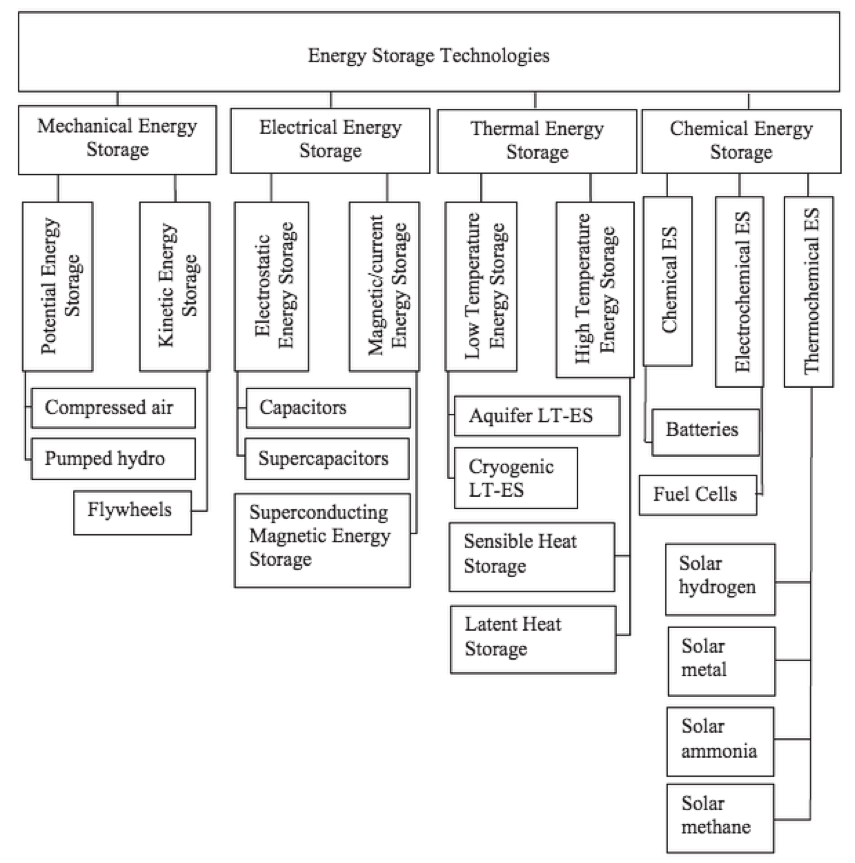
\includegraphics[scale=1.0]{pics/PatrickFigure1.png}
\caption{An impressive variety of energy storage mechanism have been studied in
parallel to the development of renewable energy generation.[1] }
\label{p1}
\end{center}
\end{figure}

Of these solutions, Compressed Air, Pumped Hydro, Flywheels,
Capacitors/Supercapacitors, Sensible Heat Storages, and Batteries are
considered ready to deploy on a commercial scale.[1] Each of these technologies
is evaluated below for their usefulness in storing energy generated by
photovoltaics for use in government buildings. In order to give the reader a
sense of scale when considering the power capacities of these technologies, the
following information is reported by the Energy Information Agency:
\begin{itemize}
\item There are a total of 84,000 government buildings in the country, together
consuming approximately .093 Quadrillion BTU annually.
\item Therefore, an average government building uses an average of .037 MW
throughout a 24-hour period.
\item There are 41,000 Government Buildings that consume between .00208 MW and
.0104 MW on average.
\item There are 35,000 Government Buildings that consume between .0104 MW and
.104 MW on average.
\item There are 5,000 Government Building that consume more than .104 MW, and
the largest government building by square footage, the Pentagon, consumes roughly
12.6 MW.[2]
\end{itemize}

For each technology, three critical metrics are listed. Capacity refers to the
power that the technologies can continuously discharge, with upper and lower
bounds determined both by technological limitations and efficiencies of scale.
Round trip efficiency refers to the amount of electrical energy the system can
discharge as a percentage of the energy it is charged with. Capital refers to
the initial cost of equipment per unit energy of storage. These criteria
represent a snapshot of how effective and economical a given storage technology
is for a particular application.

\subsubsection{Compressed Air}
\textbf{Capacity: 3-15 MW}

\noindent\textbf{Round Trip Efficiency: 50 \%}

\noindent\textbf{Capital: 100 \$/kWh}

Compressed Air Energy Storage (CAES) operates on the principle of
pressure-volume energy, which is converted to kinetic energy upon expansion in
a turbine. Below ground CAES has been demonstrated in Germany and the US on the
utility scale, being linked to a 290 MW and 110 MW plant, respectively. The
compressed air can be stored either underground - which requires locating a
suitable cavern - or above ground in man-made pressure vessels. The statistics
given are for above ground storage, more applicable in the case of federal
buildings because they could be implemented in any location with enough space
for a compressed air tank, regardless of geology.

Compressed air has been shown to be economical and reliable on the utility
scale, and represents a relatively modest capital investment as compared to
more technologically advanced solutions. However, its applications to single
federal buildings is likely limited due to its lower bound of power capacity, 3
MW. While CAES systems as small as 25 W have been produced on the laboratory
scale, these have not been rigorously evaluated by industry and will not likely
be deployable in the timeframe this policy concerns. Only the largest federal
buildings, or perhaps connected networks of buildings, would be effectively
served by this solution.

\subsubsection{Pumped hydro storage}
\textbf{Capacity: 100-5000 MW}

\noindent\textbf{Round Trip Efficiency: 75 - 85 \%}

\noindent\textbf{Capital: 100 \$/kWh}

Pumped hydro storage is another demonstrated technology that is known to be
effective at the utility scale. However, due to the difference in elevation
required (hydroelectric power generation is very dependent on the height or
``head'' of the water above the turbine, to the 3/2 power to be precise) this
technology is much more difficult to scale down, and thus would not be
applicable to any system with a capacity less than 100 MW. Since this excludes
federal buildings, pumped hydro storage is not applicable to the policy in
question.

\subsubsection{Flywheels}
\textbf{Capacity: .25 MW}

\noindent\textbf{Round Trip Efficiency: 93 - 95 \%}

\noindent\textbf{Capital: 5000 \$/kWh}

A flywheel is a mechanism that stores kinetic energy in a rotating mass. The
most recent iterations of this technology involve a carbon-fiber wheel that
rotates on a low friction or magnetic levitation bearing for minimal energy
loss to friction. As excess energy is generated, a motor propels the flywheel,
increasing the angular momentum of the system. As energy is required, the motor
acts as a generator to convert this momentum to electricity. This technology
has been proven effective in smoothing out intermittent power production,
primarily in wind systems. An individual flywheel can only sustain discharges
for times up to 15 minutes or so, and standby losses (the flywheel losing
energy over time due to friction) limit the effective duration of energy
storage.  This is a technologically advanced solution, and the up-front capitol
costs are the greatest of any of the solutions discusses. The merits of this
technology - its proven 20 year lifespan and its ability to charge and
discharge more rapidly than most other storage solutions - mean there are niche
applications could stand to benefit from the large investment.


\subsubsection{Supercapacitors}
\textbf{Capacity: 0-.3 MW}

\noindent\textbf{Round Trip Efficiency: 90 - 95 \%}

\noindent\textbf{Capital: 2000 \$/kWh}

Unlike the above solutions that necessitate the conversion of electrical energy
to mechanical energy and back, supercapacitors operate by storing energy in an
electric field. They entail a lower capitol expense than flywheels while
maintaining a similar efficiency and capacity. They also are expected to have a
20 year lifespan with continuous charging and discharging, and are able to
operate between -40$\degree$F and 160$\degree$F, encompassing temperatures they
would likely be exposed to in the US. Since the total energy storage of a supercapacitor is:
\begin{equation}
W_{eff}=\frac{C}{2}*(V^2_{max}-V^2_{min})
\end{equation}

The storage necessary can be scaled as needed for the application by varying
capacitance (C). One drawback is that supercapacitors can only effectively
discharge for one hour, so it is unlikely that a single supercapacitor would be
able to serve the needs of a federal building. The utilization of
supercapacitors requires advanced power electronics, which add complication and
expense. Ultimately, their hardiness can justify this expense in extreme
environments where cheaper forms of storage aren't reliable.


\subsubsection{Thermal Storage}
\textbf{Capacity: 0-60 MW}

\noindent\textbf{Round Trip Efficiency: 30-60 \%} 

\noindent\textbf{Capital: 100 \$/kWh}

The thermal storage of energy can take several forms. It can operate at high
temperatures or cryogenic temperatures, and can store energy in the form of
latent heat of phase transformation or sensible heat stored in a single-phase
medium. High temperature, sensible heat storage systems are the most developed,
and can be based around materials such as graphite, hot rocks, and molten salt.
A heat pump is used to input thermal energy to these media, and the energy is
discharged to produce supercritical steam in a conventional steam generator.
This method requires a lower investment in terms of development and
manufacturing than other thermal storage methods.
 
As compared to flywheels and supercapacitors, thermal storage can have very
long sustained run times, up to 24 hours or more. In relation to powering
federal buildings, this means that fewer thermal storage systems would be
required to power the structure over extended periods of solar deficit. A
molten salt storage scheme was shown to be effective in the Solar Two project.
In Solar Two, molten salt was used as a thermal storage mechanism, and 99\% the
thermal energy was effectively converted to electricity, as compared to
generating electricity directly from the heat of the solar input.[3]
Furthermore, while the use of this technology requires the development of a
physical storage system, it has been demonstrated that such systems can be made
on ``roof-top scale'' for ``micro-utilities'', and these systems are characterized
by energy densities similar to lithium-ion batteries.

\subsubsection{Batteries}
\textbf{Capacity: 0-40 MW}

\noindent\textbf{Round Trip Efficiency: 60 - 90 \%}

\noindent\textbf{Capital: 400-2500 \$/kWh}

A wide variety of batteries have been developed for energy storage
applications. Some of these include, in order of increasing round-trip
efficiency, Ni-Cd, Pb-Acid, Na-S, and Li-ion batteries. In general, they are
expected to be functional for between 2000 and 4500 charge-discharge cycles, or
between 5 and 13 years if they undergo one cycle per day. This is about half of
the expected lifetime of storage systems, so there is an increased long-term
investment related to system upkeep. Furthermore, all the batteries listed
require either heating or air conditioning to maintain functionality. If
they're utilized in an environment that would require a significant amount of
energy to maintain operating temperature, this is yet another associated expense.

One advantage that batteries present is their energy density. Of the solutions
discussed so far, thermal energy storage has the greatest energy density, at 80
- 200 watt hours per kilogram. Li-ion batteries have a similar energy density
(75 - 200 Wh/kg) while Na-S batteries have an increased energy density (150-240
Wh/kg), and both are approximately twice as energy efficient as thermal
storage.

\subsection{Evaluation}
The necessary storage capacity of any given building was estimated under a
``worst case scenario'' set of assumptions. Namely these are:
That the buildings will run exclusively off of generated photovoltaic power?

The evaluation of these technologies was based on two central aspects. First,
the storage demand for any given federal building was estimated based on its
average power capacity and the ability of its environment to support solar
power. Second, the total cost of installing and operating each of the storage
systems listed for 20 years was estimated as a function of storage capacity
installed. Thus, the lowest-cost solution for any given capacity can be
indicated. Third, special considerations that may impact the choice of a
storage technology, such as climate, required responsiveness, and limited
space, were identified and matched with an appropriate technology.

\subsubsection{Estimating storage demand}

To estimate the needed storage demand, the problem to be solved must first be
defined. In this case, it's not so much a matter of evening solar output vary
from day to day, but evening it out over the course of the day. The base-line
utilities know what the basic load profile will look like depending on the
region and the time of year. If they can predict 24 hours in advance how much
solar power will need to be compensated for, they can ensure that the total
energy demand is met. The problem comes when, for instance, a sunny day is
expected and a cloudy day occurs instead. In this case, the base-line utilities
can be sluggish in their response. If the output of photovoltaic sources on the
grid were to drop by more than approximately 5\% per hour, the utilities would
not be able to respond effectively and power demand would not be met. This corresponds to:

.037 MW per building, 28 buildings per county on average, 5\% of X\% (capacity)
of this product is .052*X MW/hour.

In a worst case scenario, the utilities will have planned on a perfectly sunny
day, with a output profile shown by a solid blue line in figure 2 below. At
some point during the day, PV output will drop to zero and energy storage will
have to compensate for the rest of the day. If the output of the PV/Storage
system drops by 5\% each hour until the projected power output is met again it,
the output of the PV array would look like the blue dashed line below and the
storage output would look like the red output in fig. \ref{p2}

\begin{figure}
\begin{center}
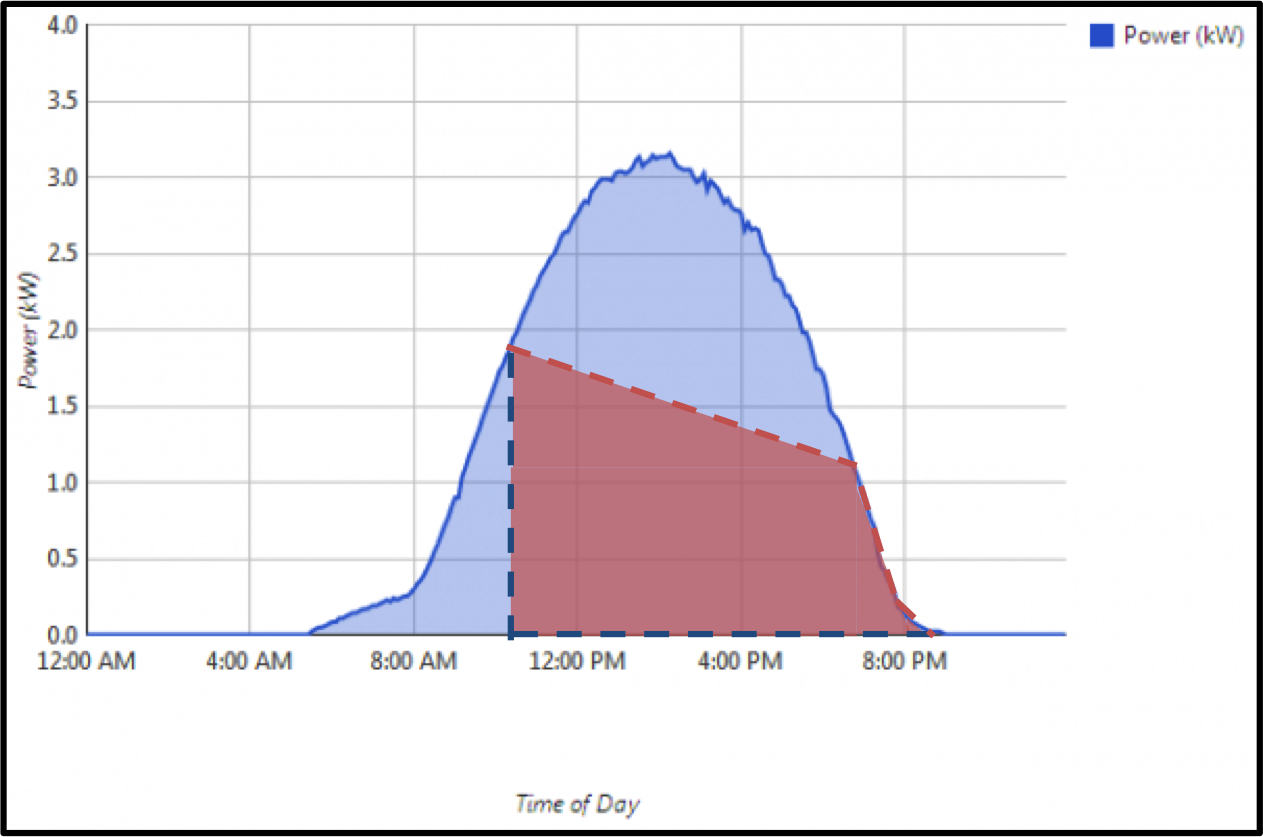
\includegraphics[scale=0.6]{pics/PatrickFigure2.png}
\caption{Storage output.}
\label{p2}
\end{center}
\end{figure}

Therefore, the area under the dashed red line, hightlighted in red, represents
the total energy storage required to get through the day. For such a geometry,
the maximum area under the curve will be roughly 56\% of the total energy
capacity of the PV system, the area under the solid blue line. In terms of
energy storage, this means that approximately 56\% of a system's daily output
must be stored to maintain the integrity of the grid in a ``worst case scenario''
day.

According to the Stefan-Boltzmann law describing radiation from a blackbody:
\begin{equation}
j^* = \sigma T^4
\end{equation}

Where T is absolute temperature [K], $\sigma$ is a constant equal to 5.670*10-8
$\frac{W}{m^2*K^4}$, and $j^*$ is the energy radiated per unit surface area of
the blackbody.
Assuming a steady state where incoming flux to the blackbody is equal to
outgoing flux and accounting for the albedo of the earth:
\begin{equation}
T={(\frac{j^*}{\sigma})}^{1/4}=(\frac{j_o(1-albedo)}{\sigma})^{1/4}
\end{equation}

Where jo is the flux, and albedo of the earth is approximately 0.3. Solving for
incoming flux:
\begin{equation}
j_o=T^4*\sigma*1.429
\end{equation}

If flux is proportional to the output of a photovoltaic array under that flux:
\begin{equation}
\frac{j_{o,1}}{j_{o,2}}=\frac{output_1}{output_2}=\frac{T_1^4}{T_2^4}
\end{equation}
If output2 is assumed to be on a cloudy day (worst case scenario), then a more
accurate relationship would be:
\begin{equation}
\frac{j_{o,1}}{0.4j_{o,2}}=\frac{output_1}{output_2}=\frac{T_1^4}{0.4T_2^4}
\end{equation}
\begin{equation}
\frac{output_1}{output_2}=\frac{T_1^4}{0.4T_2^4}
\end{equation}

Since solar panels can only utilize 40\% of diffuse irradiation. If we want a
97.8\% chance that there will be enough storage capacity on any given day, we
can find the percentage in output that needs to be stored. Assuming that T1 is
the average temperature of the lower 48 states, 284.6 K, and that output1 is
the maximum output of any given day.

\begin{equation}
\begin{aligned}
\frac{output_{max}-(\text{PV output}_2+\text{storage output})}{output_{max}} &=
\\
1-.4\frac{(284.6[K]-2*stddev)^4}{(284.6[K])^4}-\frac{storage}{output_{max}}
&=.45
\\
\end{aligned}
\end{equation}
 
where ``stddev'' is the standard deviation of
temperature at the building location, which can be taken from fig. \ref{p3}
below.

\begin{figure}
\begin{center}
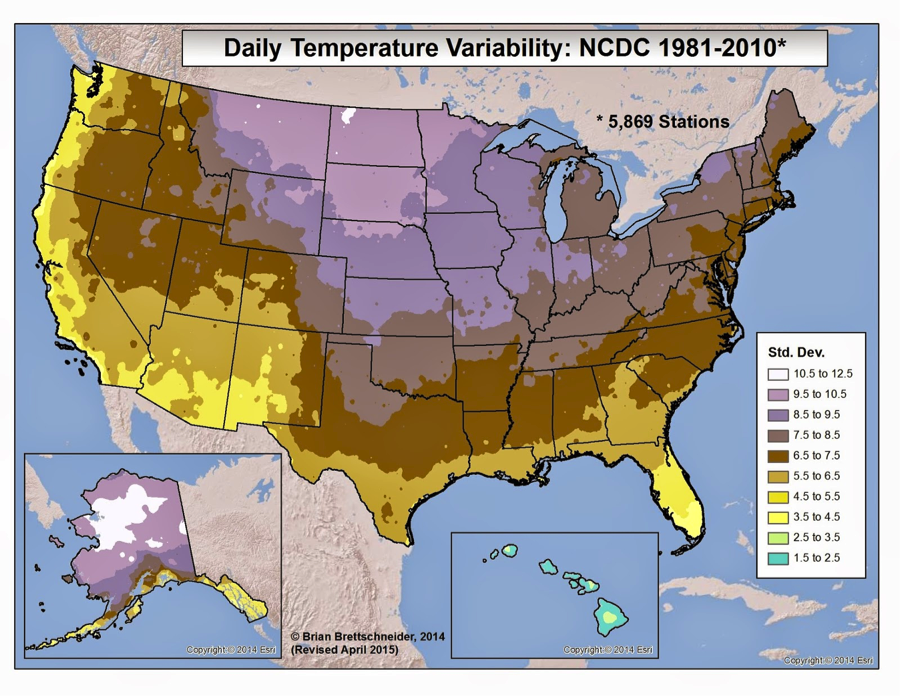
\includegraphics[scale=1.0]{pics/PatrickFigure3.png}
\caption{Daily Temperature Variability}
\label{p3}
\end{center}
\end{figure}

Solving for the necessary storage as percent of capacity:
\begin{equation}
.55-.4\frac{(284.6[K]-2*stddev)^4}{(284.6[K])^4}=\frac{storage}{output_{max}}
\end{equation}

The amount of storage needed to handle the worst case scenario day one and the
second worst case scenario day two will also depend on whether or not the
storage will be able to recharge in the interim. This is effectively a function
of how likely a sunny day is at the building site. At any given location on the
globe, there are 4383 hours of daytime (and 4383 hours of night) per year.
Assuming that 5\% of the PV energy generated is diverted to storage during any
given hour, approximately 11 hours would be needed to recharge the storage
system that supports 56\% of the total daily demand. In a worst case scenario
(at the northern fringe of the continental US on the winter solstice), there
are approximately 9 hours between sunrise and sunset. So at most, 45\% of daily
capacity could be stored in such a scenario. This means that at least an
additional 10\% of daily capacity would have to be accounted for in pre-stored
energy, and 55\% at most. The calculation of average hours of sunlight in 9
hours of daytime is fairly straightforward:

\begin{equation}
hrs_{sun,avg}=\frac{hrs_{sun,annual}}{4383 [hrs]}*9 [hrs]
\end{equation}

Using this expression to estimate the percentage of daily capacity that may be
expected to regenerate:

\begin{figure}
\begin{center}
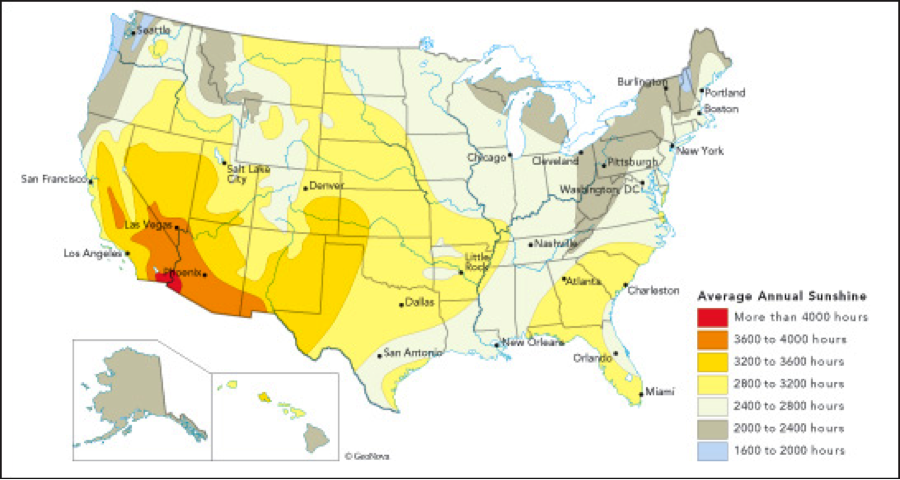
\includegraphics[scale=1.0]{pics/PatrickFigure4.png}
\caption{Average Annual Sunshine}
\label{p4}
\end{center}
\end{figure}

\begin{equation}
\frac{storage_{required}-storage_{regenerated}}{output_{max}} =
.55-.05*\frac{hrs_{sun,annual}}{4383} [hrs]*9
\end{equation}

Thus, calculating the total storage needed for this worst case scenario:
\begin{equation}
\begin{aligned}
\frac{Storage}{output_{max}}&=storage_{Day1}+storage_{Day2}-expected
regeneration
\\
&=.55+.55-.4\frac{(284.6[K]-2*stddev)^4}{(284.6[K])^4}-.05*\frac{hrs_{sun,annual}}{4383
[hrs]}*9 [hrs] \\
&=1.1-.4\frac{(284.6[K]-2*stddev)^4}{(284.6
[K])^4}-.45*\frac{hrs_{sun,annual}}{4383}  \\
\end{aligned}
\end{equation}
\begin{equation}
Storage=output_{max}(1.1-.4\frac{(284.6[K]-2*stddev)^4}{(284.6
[K])^4}-.45*\frac{hrs_{sun,annual}}{4383})
\end{equation}

Capturing the influence of the building location on the necessary storage capacity:
\begin{equation}
\text{Environmental Factor}=1.1-.4\frac{(284.6[K]-2*T_{stddev})^4}{(284.6
[K])^4}-.45*\frac{hrs_{sun,annual}}{4383})
\end{equation}

\subsubsection{Evaluation of cost}

The average service life required for photovoltaic panels to pay themselves off
is 15-25 years. Conveniently, all of the storage mechanisms listed will last 20
years, excepting batteries which last an average of 10 years or so with daily
cycling. Given these facts, 20 years was chosen as a time frame over which to
estimate the cost of capital, installation, and maintenance for each energy
storage solution.

\begin{figure}
\begin{center}
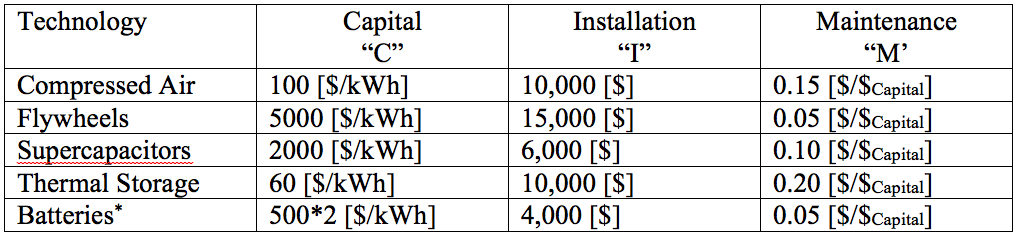
\includegraphics[scale=0.3]{pics/PatrickTable0.png}
\caption{Based on Sodium-Sulfur batteries, which we judged to be the most
reliable, efficient, and suitable in this application.}
\label{patrickTable0}
\end{center}
\end{figure}

So, the 20 year cost can be calculated as:
\begin{equation}
\begin{aligned}
Total cost&=Capital+Installation+Maintenence\\
Total cost&=(C[\frac{\$}{kWh}](1+M[\frac{\$}{\$}])*Capacity[kWh])+I\\
\end{aligned}
\end{equation}

This function is graphed below for each of the five proposed storage
technologies. Note that flywheels and compressed air both have a minimum
threshold capacity, and are plotted only over the capacity range in which they
are feasible.

\begin{figure}
\begin{center}
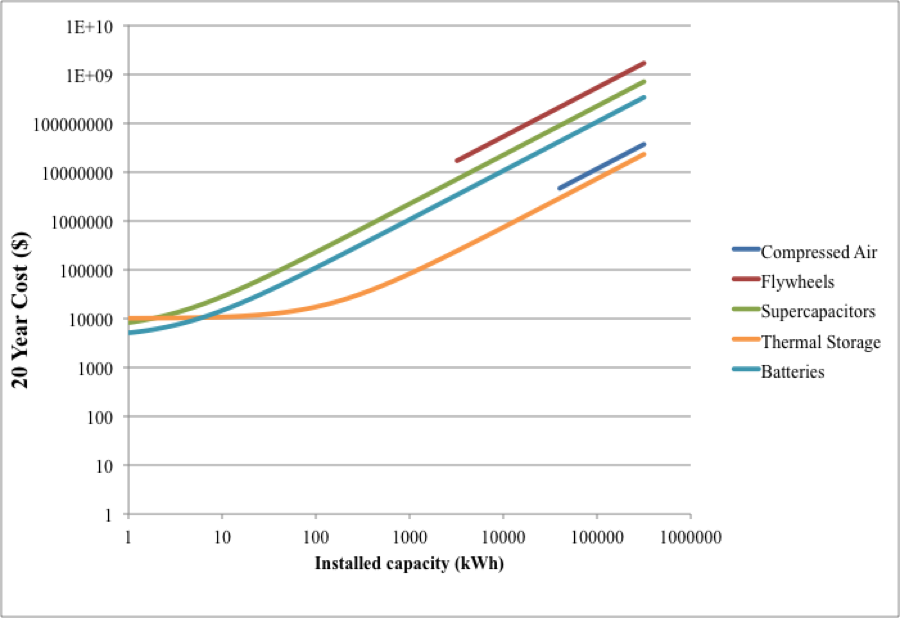
\includegraphics[scale=1.0]{pics/PatrickFigure5.png}
\caption{20 year cost}
\label{p5}
\end{center}
\end{figure}

Thus, Sodium-Sulfur batteries are expected to be most affordable for storage
capacities below 7 kWh, and thermal storage for capacities above 7 kWh. Using
this data, the most economic storage mechanism can be identified as a function
of environmental factor and the installed PV capacity required by the policy (a
certain percentage of total energy demand, depending on the date of
construction or retrofitting). These results are summarized below:

\begin{figure}
\begin{center}
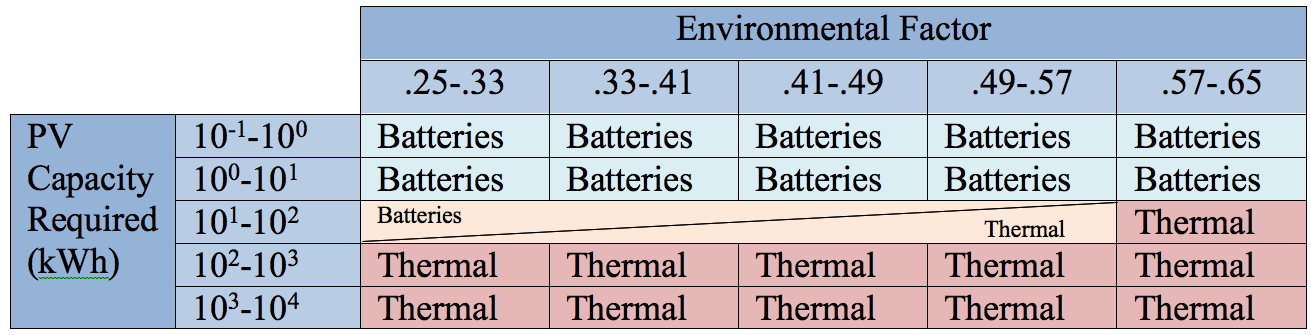
\includegraphics[scale=0.3]{pics/PatrickTable1.png}
\caption{Environmental Factors}
\label{patrickTable1}
\end{center}
\end{figure}

If this is applied to Greve Hall, with a daily energy consumption of $=4.285*103
kWh$ and an environmental factor, E, 
\begin{equation}
\begin{aligned}
E &=(1.1-.4\frac{(284.6[K]-2*7.2)^4}{(284.6[K])^4}-.45*\frac{2400}{4383})\\
&=.56681\\
\end{aligned}
\end{equation} 
Indicating that a thermal storage system would be the most affordable solution.

Of course, not all storage scenarios can be fully described by two numbers. In
some cases, there will be particular demands or constraints that may
necessitate the use of a more expensive storage technology. These include:
\begin{itemize}
\item Situations in which the photovoltaic array represents a very significant
portion of the total grid input, and the ability of the storage system to
compensate for PV loss within a few milliseconds is important. In this case,
flywheels have been demonstrated to have very quick ramp-up and ramp-down rates
in conjunction with solar systems.
\item Situations in which temperature extremes are expected and it's not
feasible to control the storage system's environment. Supercapacitors stand out their abity
to operate between -40$\degree$F and 160$\degree$F for long cycle lifetimes.
\end{itemize}

\subsection{Conclusions}

Can today's demonstrated energy storage solutions effectively and economically
deliver power to federal buildings as needed, given the intermittent nature of
solar power generation? We believe that the data here presented evidences that
they can. For any given combination of environment and PV capacity, one of two
energy storage solutions is the most viable. This elegant result will simplify
the installation of the PV array/storage system and allow costs to be
minimized. In terms of cost, it is worth noting that the cost of thermal energy
storage is approximately \$300 per kW, and as low as \$300 per kW in battery
systems. Given that the photovoltaic arrays here discussed cost on the order of
\$2,000 per kW, this additional cost is non-negligible, but extremely reasonable
to ensure the reliability of the grid.

Furthermore, while alternative solutions to intermittency could be established,
such as on-site generation using existing natural gas sources, this policies
commitment to carbon neutrality heavily favors the philosophy of energy
storage. In addition to stand-alone storage systems, rechargeable electric
vehicles could also fill the role of intermittency mitigation. This possibility
is discussed in another section.

\bibliographystyle{patrick}{ieeetr}
\bibliography{patrick}{patrick}{References}
\clearpage

% ----- Eric ----- %
\newbibliography{eric}
\section{Using Solar Energy to Power a Federal\\ Electric Vehicle Fleet}

\emph{Eric Muckley}







\subsection{Introduction}

In order to reduce its dependence on fossil fuels and reduce GHG emissions, the U.S. must abandon a transportation paradigm that relies on the use of internal combustion engines (ICEs). As world petroleum reserves are depleted and the price of gasoline inevitably rises, it is likely that electric vehicles (EVs) and hydrogen fuel cell vehicles (FCVs) will replace ICE vehicles as dominant modes of personal transportation. Although FCVs exhibit some clear performance advantages over EVs, existing national infrastructure strongly favors the adoption of EVs over FCVs~\cite{eric}{20}. For this reason, the discussion presented here will focus on the adoption of EVs and hybrid EVs rather than FCVs.  


It is well known that large-scale adoptions of both solar energy and EVs are currently limited by technological and economic problems. The intermittency of solar power generation and the lack of a suitable storage solution for excess production, as well as the high cost of photovoltaics (PVs), has prevented solar energy from becoming a significant source of electricity generation in the U.S. Similarly, the strain that large EV fleets place on the electric grid, as well as their high carbon footprint if powered by electricity from coal, have presented roadblocks to wide-scale adoption. In this discussion, it is demonstrated that the increase of solar energy generation at federal facilities presents a unique opportunity for an economically viable, large-scale implementation of electric vehicles (EVs) into the federal vehicle fleet.

There are significant advantages to coupling the large-scale adoption of EVs with an increase in solar energy generation. Storing excess solar energy in EV batteries can help mitigate the energy storage problem posed by solar energy production, and recharging EVs using solar energy is significantly less expensive than refueling using gasoline. Charging EVs with solar energy reduces both the nation's dependence on fossil fuels and the amount of GHGs emitted by the transportation sector. Coupled with the large-scale federal adoption of energy generation from PVs, a shift towards widespread federal EV usage can make both EVs and PVs commercially feasible by increasing demand in EV and PV markets without enacting costly government subsidies.





\subsection{EV Deployment into the Federal Transportation Fleet}

A decision by the U.S. government to take a leadership role in EV adoption would result in a reduction in national GHG emissions, improvement in the country's energy independence, creation of high-quality jobs, and foster economic growth~\cite{eric}{million}. To help establish the U.S. as a leader in EV usage, in 2011 President Barack Obama set a goal to have one million EVs on U.S. roads by 2015. His plan was to support the EV industry through new tax credits, increases in R\&D expenditures, and investment in programs which aim to develop the infrastructure required for large-scale EV adoption~\cite{eric}{million}. However, it is well into 2015 and the U.S. has only 300,000 EVs on the road~\cite{eric}{third}. President Obama's plan to accelerate growth in the EV marketplace has failed because despite subsidies for EV purchases, consumer demand remains low~\cite{eric}{million}. Rather than paying consumers large subsidies, federal agencies have increased EV demand by purchasing EVs for use in their own transportation fleets. Federal purchase of EVs helps expand the domestic EV market by increasing the demand for EV technologies and services, which in turn drives down the cost of EVs and makes them more economically appealing to the general public. More importantly, this approach can be accomplished without imposing costly federal EV subsidies. The U.S. government currently owns or leases over 635,000 automotive vehicles for transportation purposes, which consume the equivalent of about 300~million gallons of gasoline each year, costing roughly \$1.3~billion annually. Only about 0.02\% of this cost is spent on electricity for recharging EVs in the federal fleet~\cite{eric}{fleetreport}. 

Between 2009 and 2013, the U.S. government purchased and leased an average of about 50,000 new federal fleet vehicles per year. Of the 45,000 new vehicles purchased in 2013, over 90\% were gasoline, diesel, or flexfuel-powered~\cite{eric}{fleetreport}. By limiting EV purchase to less than 1\% of its total vehicle fleet, the U.S. government has traditionally withheld support for the growth of domestic EV industries and failed to capitalize on opportunities to reduce GHG emissions and national dependence on foreign oil. 


Besides fostering growth of the domestic EV marketplace, implementing EVs as federal fleet vehicles would also help federal agencies satisfy the guidelines set by Executive Order 13514, which was issued by President Obama in 2009. This order requires federal agencies to reduce GHG emissions, reduce fleet petroleum consumption by 30\% before 2020, and leverage federal purchasing power to promote environmentally-responsible products and technologies~\cite{eric}{fleetemission}. The order also stipulates that 95\% of all federal contracts must meet sustainability requirements. Enacting a plan for EV incorporation into the federal transportation fleet enables significant progress toward achievement of the goals presented by Executive Order 13514, especially in the context of emissions abatement, petroleum usage reduction, and investment in sustainable technologies.

Since Obama began his initiatives to decrease U.S. dependence on ICEs for transportation, the number of EVs in the federal fleet has grown from 57 in 2009 to 4,000 in 2013, and the number of fleet hybrids has increased from 1,800 to 16,000 during the same time period. While this significant increase in EV usage represents important progress towards meeting federal mandates, it also causes problems. Increasing EV usage without implementing a sufficient amount of renewable energy generation means that the electricity used to recharge EV batteries must be produced from fossil fuel-burning power plants. In addition to increasing GHG emissions, this also increases the nation's dependence on fossil fuels. 




\subsection{Emissions Abatement by EV Adoption}

One of the primary drivers for large-scale EV adoption is the effort to reduce pollution and GHG emissions from vehicles. However, it is clear that even widespread EV use will not significantly reduce national GHG emissions if the electricity used to recharge the EVs is produced by burning fossil fuels. This means that increasing the generation capacity of renewable energy sources like solar and wind will have a significant effect on the effectiveness of EV implementation to improve air quality. Since renewable energy generation alone cannot help the U.S. reduce its dependence on oil for transportation, there are clear advantages to developing renewable energy infrastructure in tandem with EV adoption. Only by charging EVs using electricity generated from renewable sources can the U.S. reduce both national GHG emissions and its dependence on fossil fuels.

The effect on air quality of shifting to an EV-based transportation paradigm should not be underestimated. ICE vehicles used for personal transportation are responsible for over 40\% of the nonmethane organic gases (NMOGs), 57\% of the nitrogen oxides (NOs), and 82\% of the carbon monoxide (CO) in urban air pollution~\cite{eric}{emission}. Using the 1995 U.S. emissions standards for ICE vehicles, replacing an ICE vehicle by an EV would result in emissions reductions of NMOGs by 98\%, NOs by 92\%, and CO by 99\% per vehicle~\cite{eric}{abatement}. Decoupling the country's transportation requirements from GHG emissions can play a crucial role in mitigating climate change without imposing costly carbon taxes or other federal transportation legislation~\cite{eric}{workingpaper}. Furthermore, using solar energy to recharge EVs ensures that the vehicle emissions are not merely being transferred to the site of a fossil fuel-burning power plant, but are truly being replaced by a clean renewable energy source. This makes it especially important that increases in EV usage are closely tied to renewable energy production.


\subsection{EVs and Solar Energy Generation}


The development of a large federal EV fleet for transportation at and between federal facilities like military bases and national parks would strongly complement the implementation of solar infrastructure at these locations. This is partly due to the fact that solar investment payback times occur much more quickly when the electricity generated is not used solely for insertion into the grid, but for replacing gasoline to power vehicles~\cite{eric}{sierra}. Generating electricity using PVs, storing it, and consuming it on-site instead of immediately transferring it entirely onto the electricity grid has other advantages as well. Utilities commonly charge electricity producers a fee when that producer adds power to the grid. In fact, the Arizona Public Service attempted to impose a \$50 surcharge on electricity customers who produced their own power using PVs~\cite{eric}{fee}. By consuming electricity generated on-site, federal facilities can avoid grid fees collected by utilities, ultimately improving the long-term return on investment in solar energy generation systems. Since electricity generated by PVs is carried by direct current (DC), charging EVs directly from PV systems without first converting to alternating current (AC) also bypasses the need for power inversion, which typically introduces efficiency loses of at least 10\% each time the power is inverted~\cite{eric}{invert}. This makes direct charging of EV batteries by PV systems at government facilities especially attractive.

Insolation levels and real estate prices require that most utility-scale ($>$1~MW) solar plants are located in deserts far from large population centers where energy is consumed. The long-distance transmission and distribution of power from producers to consumers accounts for over 6\% of the energy lost in the United States each year~\cite{eric}{losses}. Using electricity generated on-site to recharge the batteries of electric vehicles minimizes distribution losses and results in higher net output efficiencies for generation systems. Furthermore, federal fleet vehicles which are not used as heavily as typical consumer vehicles are ideal for purely solar charging, as a small 3~kW system can provide 100\% of the power for a typical EV which drives 1,200~miles per year~\cite{eric}{sierra}.

One of the primary factors which currently limits large-scale solar energy production is the lack of a high-capacity robust energy storage platform~\cite{eric}{solarstore}. By charging electric vehicles directly from PV systems, energy storage can be accomplished using existing EV batteries without implementing other expensive storage solutions. Large-scale solar EV charging is more economical than using smaller modular systems, as a single 22~kWh solar energy car charging port with integrated lithium ion batteries can cost more than \$40,000~\cite{eric}{google, carreports}. The PV-EV recharging approach at government facilities advances multiple goals. It increases the market for EV and PV adoption while offering a storage solution for convenient energy retrieval without introducing loses from transmission through complex distribution networks and multiple power inversions. 


One of the reasons that federal facilities present a unique opportunity for PV-EV coupling is that electricity demand and intensity of vehicle usage undergo significant variations throughout the week. While EVs in the federal vehicle fleet may be driven frequently on weekdays, the majority of fleet vehicles are underutilized on weekends, after work hours, and on holidays. This trend is analogous to the electricity consumption patterns of federal facilities: weekdays during working hours electricity consumption is high, but it is low on weekends, holidays, and after working hours. This weekly pattern exhibits a trend which is highly optimized for electric vehicle charging by PV systems at federal facilities. During high electricity demand times, during peak sunlight hours on the weekdays, the solar power generated can be consumed on-site, without the need for inefficient long-distance distribution or storage. On weekends, when electricity consumption at federal facilities is low, the excess power produced can be used to directly charge EVs, which are underutilized during non-working hours, or can be transferred onto the electric grid.



\subsection{Costs and Benefits Associated with EV Adoption}

It is important to estimate the cost of significantly increasing the share of EVs in the federal transportation fleet. The average EV produced by U.S. automakers costs roughly \$35,000, which is around 40\% higher than similarly sized ICE vehicles if purchased new without federal tax subsidies\cite{eric}{40percent, shahan, 27k}. This means that replacing each ICE vehicle in the federal fleet by a similarly-sized EV will cost roughly \$10,000. Although it is clear that EV adoption requires initial financial investment, the cost represents a relatively small amount of the annual federal fleet budget. Coupled with large-scale solar energy generation at federal facilities, increased EV usage will result in significantly lower federal fleet fuel costs, lower GHG emissions from vehicles, and increased national energy independence due to decreased reliance on petroleum imports.


For an analysis of the economics of the large-scale purchase of EVs as federal fleet vehicles, it is assumed that each EV purchased by the federal government is replacing a conventional gasoline-powered vehicle. The roughly 350,000 gasoline-powered vehicles in the federal vehicle fleet currently consume about 300~million gallons of gasoline per year~cite{fleetreport}. This amounts to an average of about 860~gallons of gas per vehicle each year. Driving a typical ICE vehicle produces an estimated $9 \times 10^{-3}$ metric tons of CO$_2$ per gallon of gasoline consumed~\cite{eric}{IPCC}. If one gallon of gasoline is equivalent in energy to about 34~kWh~\cite{eric}{greet}, and traditional sources of electricity produce around $7\times10^{-4}$ metric tons of CO$_2$ per kWh~\cite{eric}{epacalc}, it can be estimated that powering an EV with electricity from fossil fuel-burning power plants produces roughly twice as much CO$_2$ as driving an ICE vehicle. However, recharging EV batteries with power produced from PVs results in a process which is nearly carbon neutral. This further demonstrates that EV adoption in tandem with increased PV generation is essential for decreasing GHG emissions in the transportation sector.

It is also useful to estimate the solar energy generation capacity required for fully charging electric federal fleet vehicles when electricity demand at federal facilities is low. American electric vehicle batteries have typical storage capacities of around 25~kWh~\cite{eric}{edmond}. If a 3~kW solar energy generation system can provide 100\% of the power for an EV which drives 1,200~miles per year~\cite{eric}{sierra}, and the average federal fleet vehicle drives roughly 7,500~miles per year~\cite{eric}{fleetreport}, it can be estimated that about a 20~kW system is required for the full recharging of each federal vehicle. During times at which solar electricity generation is higher than demand, this excess power can be stored in EVs parked at federal facilities. Although this discussion does not include an official policy recommendation for the adoption of EVs by government facilities, it clearly outlines the benefits associated with adoption of EVs into the federal fleet alongside an increase in solar energy generation. 


In 2013, the U.S. federal vehicle fleet consumed over \$1.3~billion worth of fuel. Cost of gasoline made up roughly 88\% of this cost, about \$1~billion worth, while electricity for EVs represented only about 0.02\% of the cost, roughly \$315,000. If the entire federal fleet consumed about 300~million gallons of gasoline, then each vehicle paid an average of roughly \$3 per gallon~\cite{eric}{fleetreport}. By replacing each federal ICE vehicle with an EV and charging that EV using solar power produced on-site at federal facilities, the federal government effectively saves over \$2,500 per year in fuel costs per vehicle. Only after 4~years does this cost make up the extra \$10,000 investment for purchasing EVs over conventional ICE vehicles. An analysis of the cost of replacing ICE vehicles with EVs in the electric fleet and the resulting reduction in carbon emissions and gasoline consumed is summarized in Table~\ref{table:EVplan}.




\begin{table}[]
\caption{The number of EVs which can be supported by installed solar generation capacity, the amount of money saved in gasoline fuel purchases assuming that the EVs are poweres solely by solar energy, and the emissions reduced by the EV fleet each year, assuming that each EV replaces a conventional ICE vehicle. }
\centering 
\begin{tabular}{c c c c} 
\hline 
Installed  &  Gov't EVs & Gas Savings& CO$_2$ equivalent   \\ 
[ .1 ex]
Capacity (MW) &Supported &  (millions of \$/yr) & (metric tons/yr)   \\ 
[ .1 ex]
\hline
10& 500 & 1.3 & 3,900 \\
50& 2,500  & 6.5 & 19,000  \\ 
100& 5,000  & 13 & 38,700  \\ 
250& 12,500 & 32 & 96,750 \\ 
500& 25,000  & 65 & 193,500 \\ 
\hline
\end{tabular}
\label{table:EVplan}
\end{table}





\subsection{EVs and PVs at Los Angeles Air Force Base: A Case Study}

It is instructive to study a concrete example of a facility which has employed PV systems which utilize EVs as an energy storage platform. Over the last decade, the U.S. Air Force has been especially proficient in incorporating EVs into their vehicle fleets. In 2013, the Air Force announced a program to lease 500 EVs and hybrids, costing \$20 million total~\cite{eric}{cleantech}. The program aims to further research on vehicle-to-grid (V2G) technology, which vehicle batteries to serve as mobile energy storage units which can be charged when electricity demand is low and discharged onto the grid when demand is high.

In November of 2014, Los Angeles Air Force Base (LA AFB) revealed that 100\% of their non-tactical vehicle fleet has been replaced with full EVs or hybrids. This fleet consists of 42 charging stations and vehicles, which include the Nissan Leaf, Ford C-Max, Chevy Volt, and VIA hybrid van, each of which is equipped with V2G technology. The reason that LA AFB has become the leader in V2G demonstration is that LA AFB is a leader in solar energy production, which nicely compliments the energy requirements of EV adoption there~\cite{eric}{v2g}. The EVs at LA AFB can be charged directly from solar energy, which helps alleviate the problem of energy storage from intermittent renewable energy generation. It also ensures that the energy required to operate the vehicles is truly clean, and that the vehicle emissions are not merely being transferred to the site of a fossil-fuel burning power plant.


The 42~vehicle fleet at LA AFB is estimated to be able to generate 700~kW when transferring electricity back into the grid, which is enough to power 140 homes on a summer afternoon~\cite{eric}{v2g}. Although the LA AFB V2G demonstration is currently the largest in the world, similar systems are being developed at Joint Base Andrews in Maryland and Joint Base McGuire-Dix-Lakehurst in New Jersey, and while the 42~vehicle fleet at LA AFB represents the largest federal EV fleet in the country, 8~other states have committed to putting 3.3~million EVs on U.S. roads by 2025~\cite{eric}{WH}. As the large-scale adoption of EV fleets with integrated V2G systems allows EVs to become more feasible energy storage platforms, both PVs and EVs become more economically viable solutions for the nation's energy and transportation requirements.


While the V2G system has proven to be a technologically viable option for solar energy storage, current efforts to enact larger-scale V2G schemes have met roadblocks, primarily in the political and regulatory sectors~\cite{eric}{v2g}. This fact further exemplifies the need for a coherent federal policy which can increase demand for solar energy which in turn encourages the purchase of EVs for both transportation and energy storage solutions.




\subsection{Conclusion}

To help establish and maintain itself as a leader in the adoption of clean technologies, the U.S. must embrace the use of EVs. Although subsidies for EV purchase have not been especially successful in driving growth of domestic EV markets, government purchase of EVs for use in the federal transportation fleet can increase the EV demand necessary for American EV industries to grow. However, even widespread EV usage will not result in reductions in GHG emissions or increase America's energy independence if the electricity used to recharge EVs is produced by burning fossil fuels. 

Implementing large-scale solar energy generation provides a number of unique economically and technologically-favorable opportunities for the adoption of EVs into the federal vehicle fleet. EV batteries offer one faucet of a highly desired storage solution to inherently intermittent solar energy. Charging EVs directly from solar energy generation systems while avoiding full integration into the electricity grid avoids efficiency loses stemming from multiple power inversions and long-distance distribution lines. Coupling solar energy to EV recharging also guarantees that GHG emissions from EVs are not being merely transfered to the site of a fossil fuel-burning power plant, but are truly decreasing. Finally, powering EVs with solar energy is much less expensive than purchasing gasoline for refueling ICE federal fleet vehicles. As the production of solar energy grows at federal facilities, the adoption of EVs into the federal vehicle fleet becomes more economical, convenient, and widespread. New demonstrations of V2G technology at federal facilities have shown that the combination of on-site solar power generation in conjunction with the adoption of grid-integrated EVs enables important opportunities to expand markets in both sectors while increasing domestic EV and PV demand, solidifying the U.S. as a leader in sustainable energy production and environmentally-responsible transportation solutions, and ensuring that problems such as solar energy storage can be dealt with in an innovative and economically-feasible way.

\clearpage
\bibliographystyle{eric}{ieeetr}

\bibliography{eric}{solar_policy_refs}{References}

\bibliographystyle{eric}{ieeetr}
\bibliography{eric}{eric}{References}
\clearpage

% ----- Chang ----- %
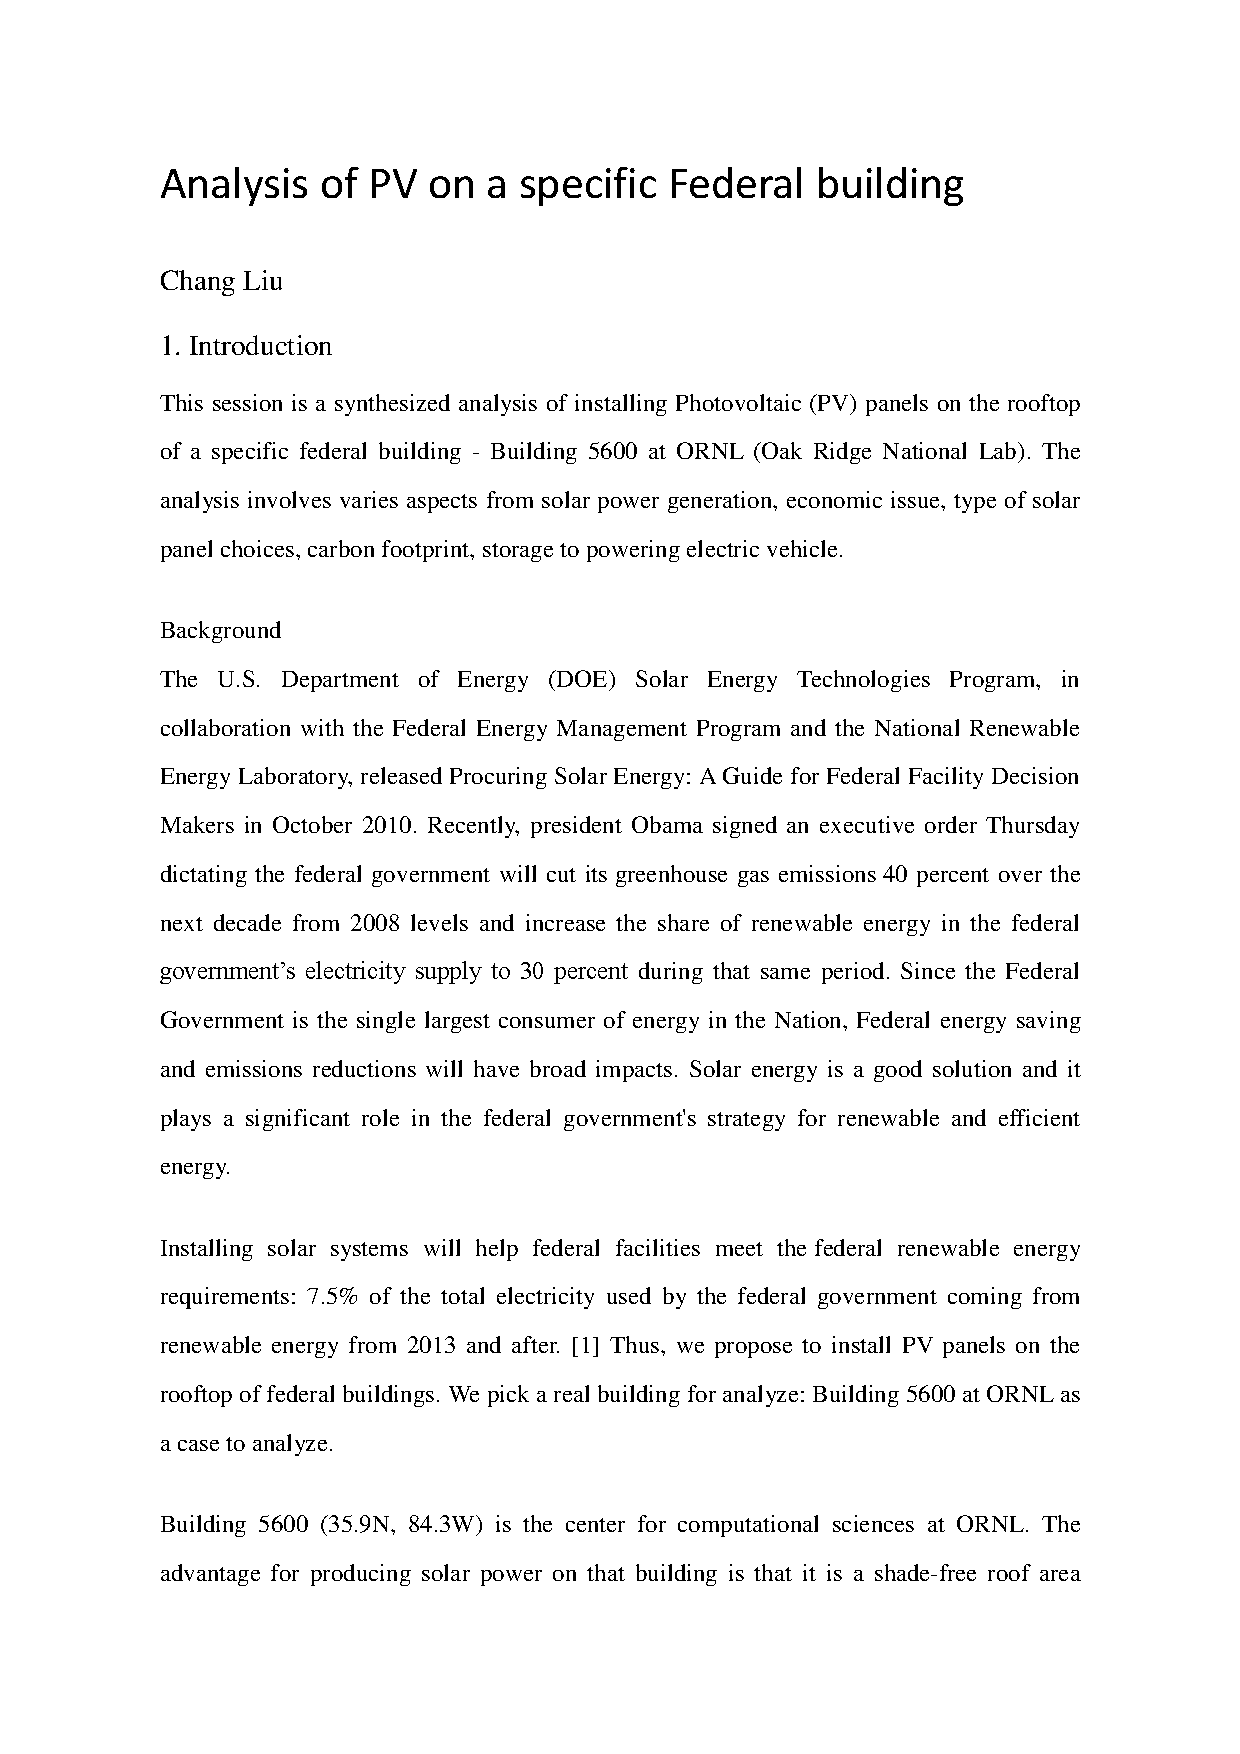
\includepdf[pages={-}]{chang.pdf}
\clearpage

\chapter{Concluding Remarks}

This policy is a progressive plan forward that is justified morally,
economically and enviromentally. Furthermore, the practical elements of such a
plan are easily achieved through implementation plans such as the ones presented
herein. It is our recommendation that such a policy be adopted with all due
haste.

\chapter*{Appendices}

%\clearpage
%\bibliographystyle{ieeetr}
%\bibliography{solar_policy_refs}
\end{document}

